\documentclass[11pt,a4paper]{article}

\usepackage[margin=2.4cm]{geometry}
\usepackage{amsmath,amssymb,booktabs,graphicx,microtype}
\usepackage{caption,subcaption,float,enumitem,xcolor}
\usepackage[hidelinks]{hyperref}
\usepackage{fancyhdr}

\graphicspath{{../figures/}}
\definecolor{accent}{HTML}{1F5A7A}
\hypersetup{colorlinks=true,linkcolor=accent,citecolor=accent,urlcolor=accent}
\pagestyle{fancy}
\setlength{\headheight}{14pt}
\fancyhf{}
\lhead{SF2956 Topological Data Analysis}
\rhead{Human activity from sensor topology}
\cfoot{\thepage}
\setlength{\parindent}{0pt}
\setlength{\parskip}{0.55em}
\setlist{nosep,leftmargin=1.4em}

\title{\textbf{Topological Signatures of Human Activity}\\
\large Persistent homology of Takens-type smartphone-sensor embeddings}
\author{SF2956 Project Group}
\date{September 2026}

\begin{document}
\maketitle

\begin{abstract}
We test whether persistent homology of short smartphone-sensor windows distinguishes six activities for unseen subjects. Each 2.56-second acceleration and gyroscope window is mapped to delay-coordinate point clouds. Vietoris--Rips barcodes in $H_0$ and $H_1$ are first sampled as stable-rank vectors. We then follow the longest $H_1$ class with a cocycle-derived circular coordinate, obtaining interpretable loop, phase-rate, and phase-linearity features for every activity. On nine held-out subjects, the 16-dimensional topology-and-dynamics vector scores 0.611 balanced accuracy, compared with 0.580 for 256 stable-rank coordinates and 0.503 after time shuffling. Its paired improvement over stable ranks is 0.031 (subject-bootstrap 95\% interval $[0.020,0.040]$). The strongest activity effects are gyroscope circular frequency, acceleration circular linearity, and acceleration longest-loop lifetime. Concatenating both topological vectors does not improve the score. Compact signal summaries score 0.852 and the supplied 561 features score 0.954. Topology therefore gives an interpretable description of periodic motion that transfers across subjects, but it is not the strongest classifier.
\end{abstract}

\section{Introduction}

A walking window and a standing window differ in amplitude, but they also differ in how their acceleration and angular velocity evolve. If the 128 samples are treated as an unordered point cloud, this order disappears. Delay coordinates instead join measurements from several times into one point. Repeated motion can then produce a different metric geometry from a static posture.

This is the representation step in the course pipeline: each datum $d$ must first become a finite set $X_d$, after which a metric, a filtered complex, and a computable invariant can be chosen \cite[Points 2--3]{course-notes}. Here $d$ is one sensor window and $X_d$ is its delay cloud. The analysis asks five questions:

\begin{enumerate}
  \item Do stable ranks of the delay clouds distinguish activities for subjects not used in training?
  \item Does any separation depend on time order?
  \item Can a persistent $H_1$ class be converted into a circular motion coordinate that distinguishes all six activities?
  \item Do the resulting topological features improve prediction, either alone or together with stable ranks?
  \item Do Euclidean and max-product sensor filtrations contain acceleration--gyroscope coupling that is absent from separate sensor clouds?
\end{enumerate}

Subject-wise validation tests transfer to new people. Instantaneous and shuffled controls test temporal order, while conventional features provide non-topological baselines. A cocycle-derived circular coordinate connects persistent loops to an estimated motion phase. A pairing control changes sensor synchronization without changing either marginal cloud.

\section{Data and sampling structure}

The UCI Human Activity Recognition Using Smartphones dataset contains 30 volunteers aged 19--48 performing walking, walking upstairs, walking downstairs, sitting, standing, and laying while carrying a Samsung Galaxy S II at the waist \cite{uci-paper,uci-repository}. Triaxial linear acceleration and angular velocity were sampled at 50 Hz. The supplied signals were noise-filtered and divided into 2.56-second windows with 50\% overlap, giving 128 samples per window.

The official split assigns entire people, rather than individual windows, to training or test data. This matters because adjacent windows overlap and measurements from the same person are dependent. Randomly splitting windows would therefore leak both subject style and shared signal samples.

\begin{table}[H]
\centering
\caption{Verified dataset structure. The two subject sets are disjoint.}
\label{tab:data}
\begin{tabular}{lrrrrrrrr}
\toprule
Split & Windows & Subjects & Walk & Up & Down & Sit & Stand & Lay \\
\midrule
Training & 7,352 & 21 & 1,226 & 1,073 & 986 & 1,286 & 1,374 & 1,407 \\
Test & 2,947 & 9 & 496 & 471 & 420 & 491 & 532 & 537 \\
\bottomrule
\end{tabular}
\end{table}

We use body acceleration and body angular velocity as two primary views. Total acceleration is excluded because it reintroduces the gravity component already removed by the dataset preprocessing and is partly redundant with body acceleration. The primary representation computes the two sensor geometries separately. A post-hoc extension first normalizes each sensor block and then joins synchronized acceleration and gyroscope delays; this avoids comparing their raw physical units directly.

\section{Topological construction}

\subsection{Takens-type representation}

Let $w$ denote one window and let
\[
a_w(i)\in\mathbb{R}^3,\qquad i=1,\ldots,128,
\]
be either its acceleration or gyroscope observation. For embedding length $m$ and delay $\ell$ samples, define
\[
\Phi_{m,\ell}(i)
=\bigl(a_w(i),a_w(i+\ell),\ldots,a_w(i+(m-1)\ell)\bigr)
\in\mathbb{R}^{3m}.
\]
The representing point cloud is
\[
X_w^{m,\ell}=\{\Phi_{m,\ell}(i):1\le i\le 128-(m-1)\ell\}.
\]
One point is therefore a short ordered motion fragment rather than one instantaneous measurement. Takens' theorem motivates delay coordinates as a reconstruction of latent dynamical state \cite{takens}; it does not guarantee reconstruction here because our signals are finite, noisy, multivariate, preprocessed, and not necessarily stationary.

We choose $\ell=15$, the first non-positive lag of the mean training-set acceleration autocorrelation. At 50 Hz this is 0.30 seconds. We begin with $m=3$, so each point lies in $\mathbb R^9$ and every cloud contains $128-2\cdot15=98$ points. Both choices are later varied without using the official test data.

The separate construction asks whether the geometry of each sensor is informative. To ask a different question---whether their synchronized evolution is informative---write $\Phi^a_{m,\ell}(i)$ and $\Phi^g_{m,\ell}(i)$ for the acceleration and gyroscope delay vectors. After normalizing the two blocks separately, define
\[
q_i^{(\lambda)}=
\left(\sqrt{\lambda}\,\widetilde\Phi^a_{m,\ell}(i),
\sqrt{1-\lambda}\,\widetilde\Phi^g_{m,\ell}(i)\right)
\in\mathbb R^{6m}.
\]
For $m=3$, the joint cloud $J_w^{(\lambda)}=\{q_i^{(\lambda)}\}_{i=1}^{98}$ has shape $98\times18$. Its squared Euclidean distance is
\[
\|q_i^{(\lambda)}-q_j^{(\lambda)}\|_2^2
=\lambda\|\widetilde\Phi^a_i-\widetilde\Phi^a_j\|_2^2
+(1-\lambda)\|\widetilde\Phi^g_i-\widetilde\Phi^g_j\|_2^2.
\]
Thus two points are close only when the two sensor histories are jointly similar. The default $\lambda=1/2$ gives the normalized sensor blocks equal weight; $\lambda\in\{1/4,1/2,3/4\}$ is tested on development subjects.

The Euclidean product permits partial compensation: a large acceleration distance can be averaged with a smaller gyroscope distance. We therefore introduce a second product metric. Write
\[
d_a(i,j)=\|\widetilde\Phi_i^a-\widetilde\Phi_j^a\|_2,
\qquad
d_g(i,j)=\|\widetilde\Phi_i^g-\widetilde\Phi_j^g\|_2,
\]
and define
\[
d_{\lambda}^{\max}(i,j)
=\max\left\{\sqrt{2\lambda}\,d_a(i,j),
\sqrt{2(1-\lambda)}\,d_g(i,j)\right\}.
\]
The maximum of two positively rescaled metrics is again a metric, so the Vietoris--Rips construction applies without modification. At equal weight,
\[
d_{1/2}^{\max}(i,j)\leq t
\quad\Longleftrightarrow\quad
d_a(i,j)\leq t\ \text{and}\ d_g(i,j)\leq t.
\]
An edge therefore appears only when the two motion fragments are close in both sensors. More generally, the two inequalities define a bifiltration indexed by separate acceleration and gyroscope thresholds; choosing $\lambda$ restricts it to a one-parameter slice, for which ordinary barcodes and stable ranks remain available. We test the same three values of $\lambda$ and call this the max-coupled filtration.

\begin{figure}[H]
\centering
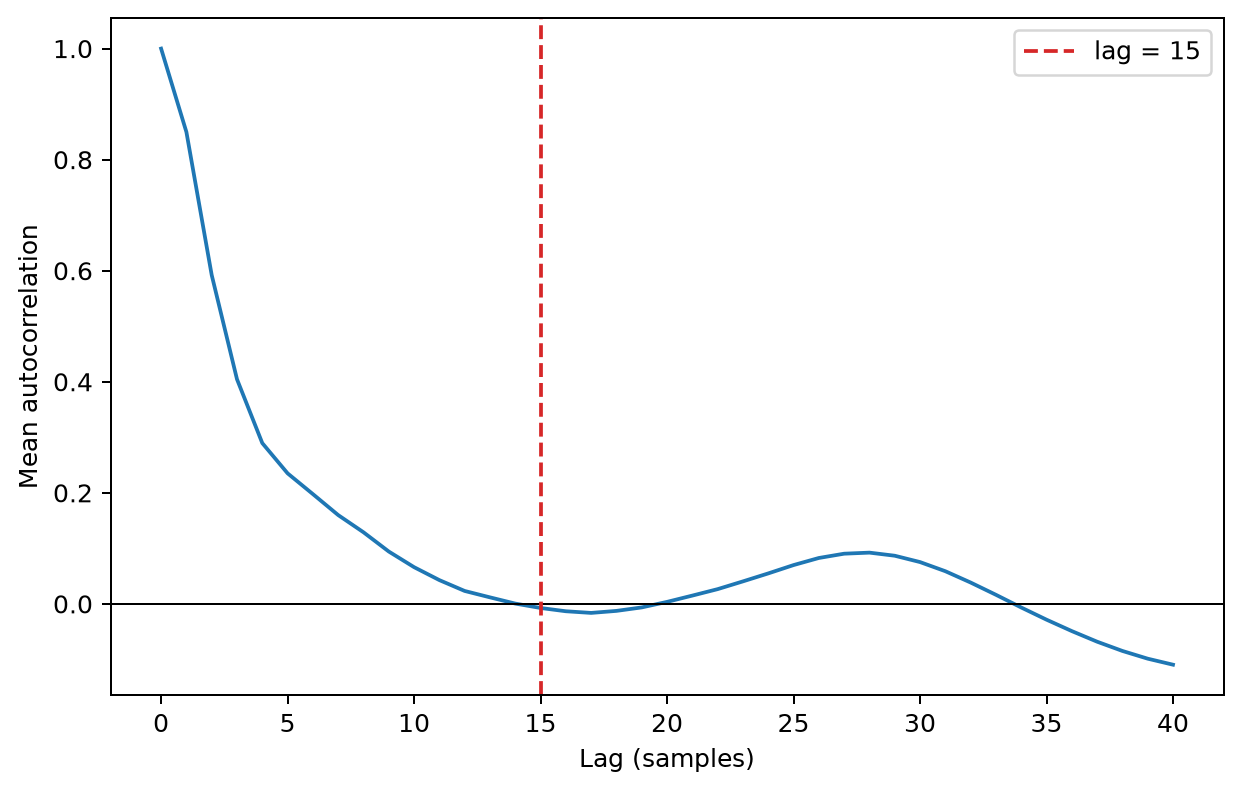
\includegraphics[width=0.72\textwidth]{autocorrelation_lag.png}
\caption{Mean normalized autocorrelation over all training acceleration windows and axes. The first zero crossing fixes $\ell=15$.}
\label{fig:acf}
\end{figure}

\subsection{Metric, scale normalization, and Vietoris--Rips filtration}

For a cloud $X=\{x_1,\ldots,x_M\}$, let
\[
s(X)=\left(\frac{1}{M}\sum_{i=1}^M\|x_i-\bar x\|_2^2\right)^{1/2},
\qquad
\widetilde X=\left\{\frac{x_i-\bar x}{s(X)}\right\}_{i=1}^M.
\]
Translation does not affect pairwise distances. Dividing by $s(X)$ removes overall amplitude so that the primary topological representation measures normalized shape. The two discarded scales are retained for a separate ablation.
More precisely, translating every point and multiplying by any nonzero scalar changes $\widetilde X$ only by a reflection when the scalar is negative. Euclidean pairwise distances, and therefore persistence, are exactly unchanged. This invariance is verified in the test suite and makes the scale ablation interpretable.

The course notes distinguish metrics from pseudometrics and emphasize that the triangle inequality is central to stability arguments \cite[Points 14--15]{course-notes}. We use Euclidean distance on $\widetilde X$ and repeat the development analysis with cityblock distance. At scale $t$, the Vietoris--Rips complex is
\[
\operatorname{VR}_t(\widetilde X)
=\{\varnothing\ne\sigma\subseteq\widetilde X:
\|x-y\|\le t\text{ for every }x,y\in\sigma\}.
\]
Points 187 and 192 of the notes define the pairwise-distance condition and the inclusions $\operatorname{VR}_s\subseteq\operatorname{VR}_t$ for $s\leq t$; Point 194 shows that the full family retains the original finite distance \cite[Points 187, 192, and 194]{course-notes}. We compute homology over $\mathbb F_2$ with Ripser.py \cite{ripser,ripserpy}. In the quotient $H_k=\ker\partial_k/\operatorname{im}\partial_{k+1}$ from Point 200, $H_0$ tracks connected components, as stated in Point 207, while $H_1$ tracks loops \cite[Points 200, 203, and 207]{course-notes}. These are loops in the reconstructed cloud, not literal circular paths of the person's body. Figure~\ref{fig:diagrams} shows one acceleration window per activity; it is an illustration, not evidence about a whole class.

\begin{figure}[H]
\centering
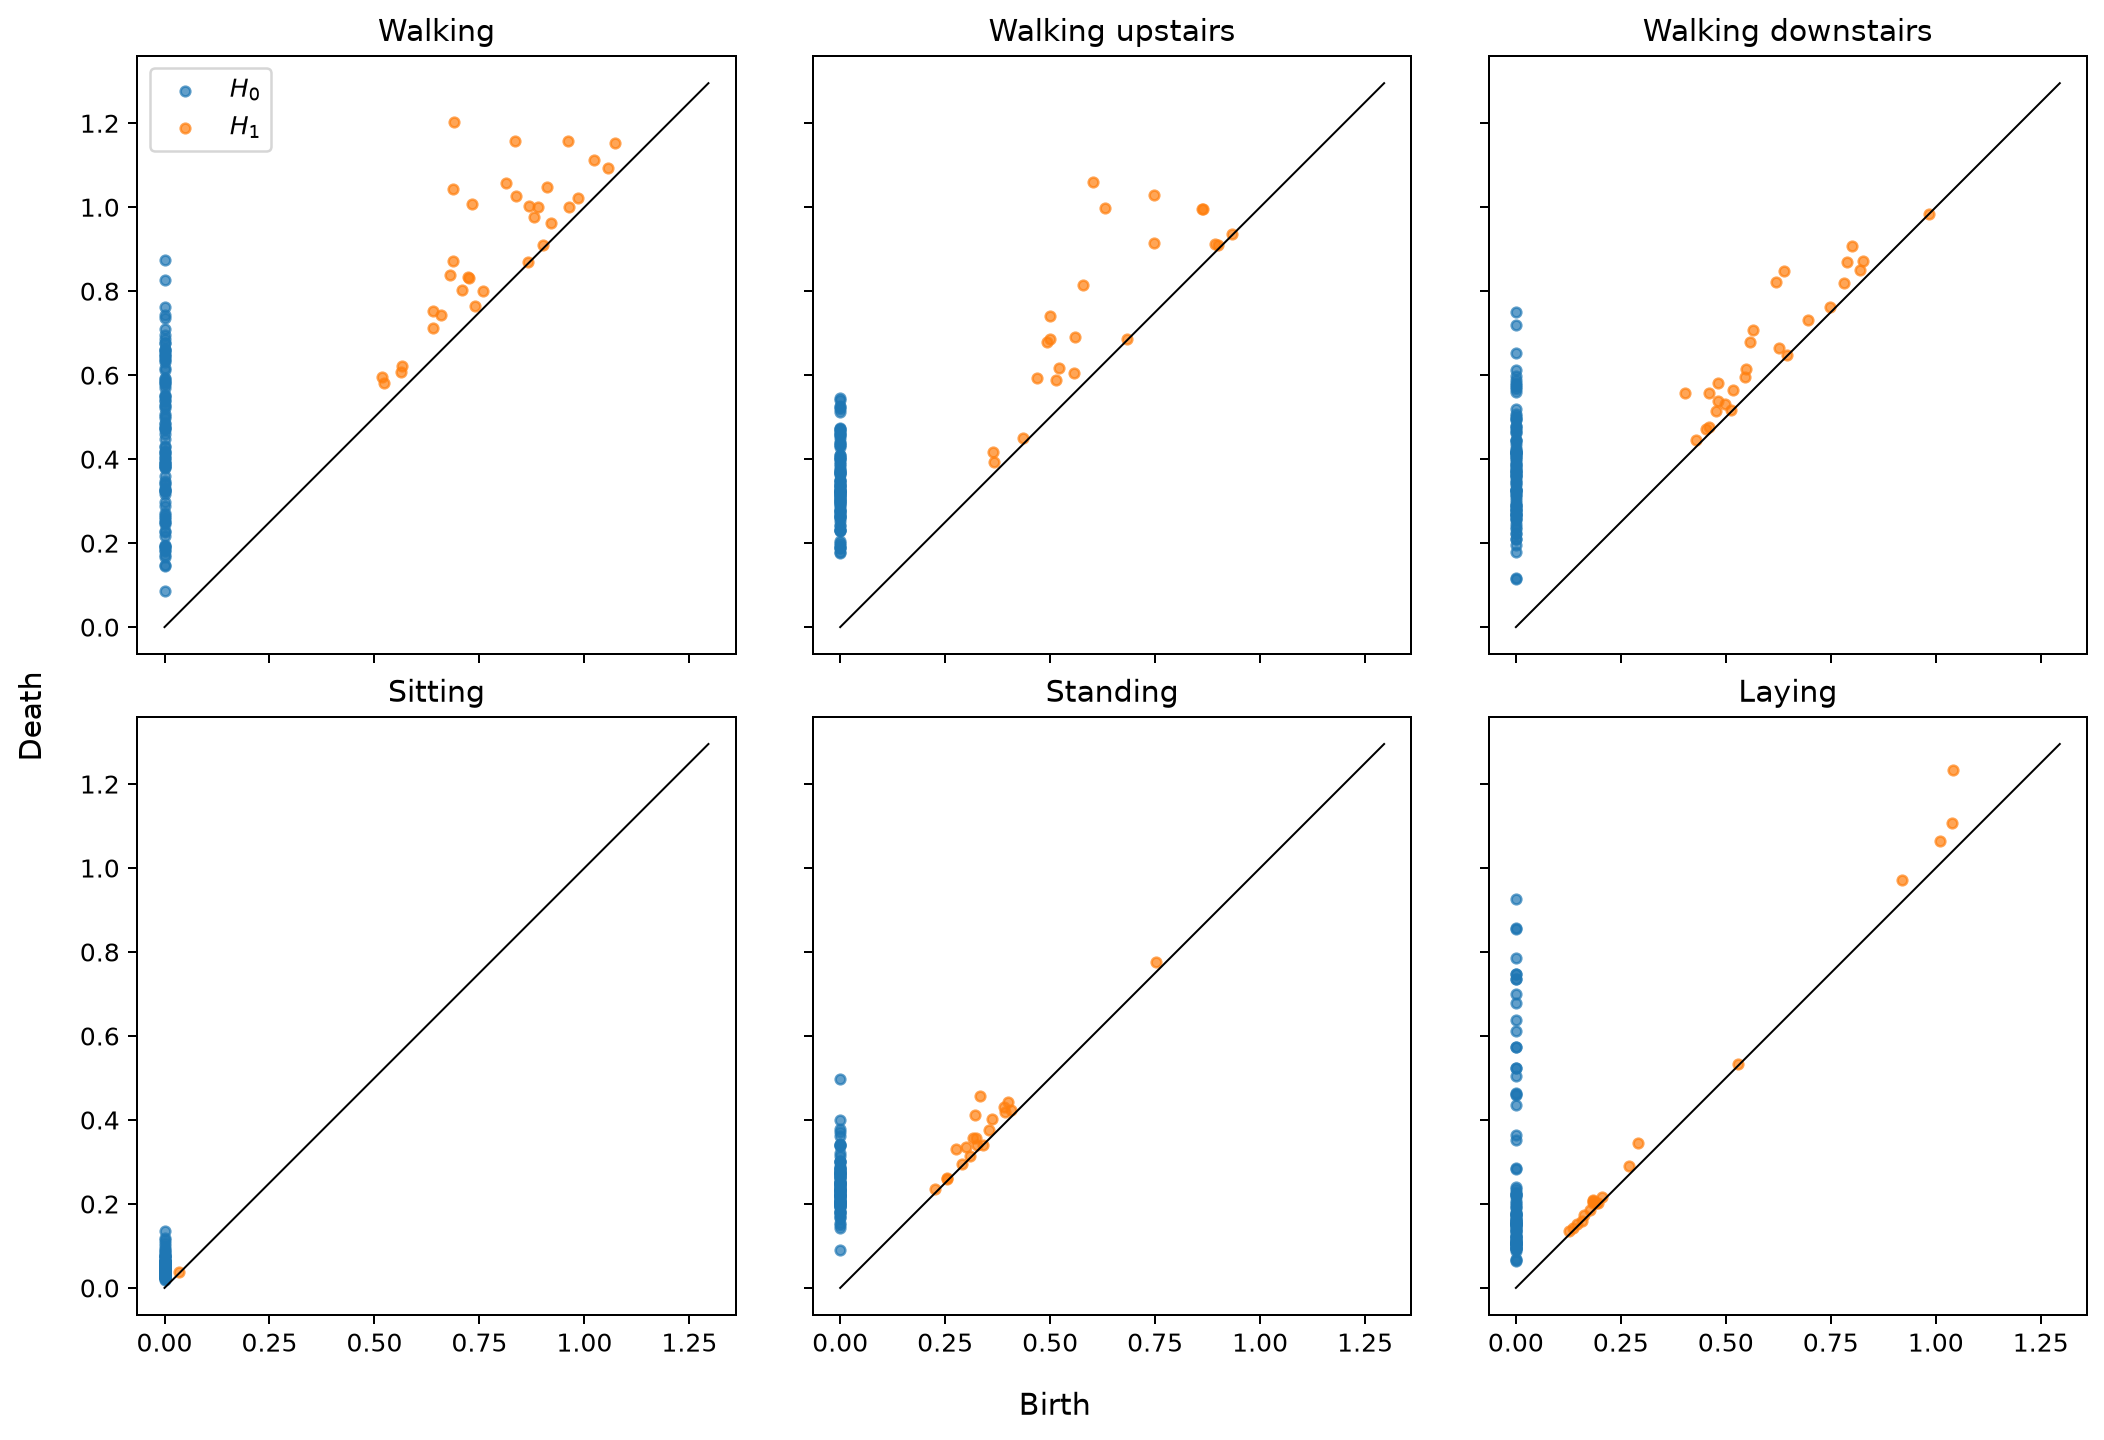
\includegraphics[width=\textwidth]{representative_persistence.png}
\caption{Representative normalized acceleration persistence diagrams for subject 1. The common axes make lifetimes comparable. The essential $H_0$ class at infinite death is omitted.}
\label{fig:diagrams}
\end{figure}

\subsection{Stable ranks}

The finite Vietoris--Rips family is tame (Point 193 of the notes). After homology it is a tame parameterized vector space, so Points 158--160 give a bar decomposition that is unique up to reordering \cite[Points 158--160 and 193]{course-notes}. A persistence barcode $B_k=\{[b_j,d_j)\}$ is then mapped to the stable-rank function \cite{stable-rank}
\[
S_k(t)=\#\{j:d_j-b_j>t\},\qquad t\ge0.
\]
It counts features whose lifetime exceeds $t$ and deliberately discards their birth positions. We compute it with StableBear \cite{stablebear}. The essential $H_0$ interval is removed so that $S_0(t)$ tends to zero. The supplied course notes take the pipeline through homology; stable rank is the additional barcode vectorization used here.

For each sensor, $S_0$ and $S_1$ are sampled at 64 equally spaced thresholds in $[0,2]$. Concatenating both homology degrees and both sensors gives the primary vector
\[
z_w^{\mathrm{sep}}\in\mathbb R^{256},
\]
ordered as acceleration $H_0,H_1$ and gyroscope $H_0,H_1$. Applying the same construction to the single joint cloud gives
\[
z_w^{\mathrm{joint}}=[S_0^{\mathrm{joint}}\mid S_1^{\mathrm{joint}}]
\in\mathbb R^{128}.
\]
Their concatenation lies in $\mathbb R^{384}$. Whenever we compare two vectors directly, the Riemann sum approximates the truncated function distance
\[
d_{[0,2]}(S,T)=\int_0^2 |S(t)-T(t)|\,dt.
\]
All $H_1$ curves are zero at $t=2$; only 30 of 10,299 windows have a nonzero endpoint in either $H_0$ block. The truncation therefore affects few windows, but we retain the notation $d_{[0,2]}$ rather than claiming the full integral over $[0,\infty)$. Figure~\ref{fig:ranks} shows class means on the 21 development subjects.

\begin{figure}[H]
\centering
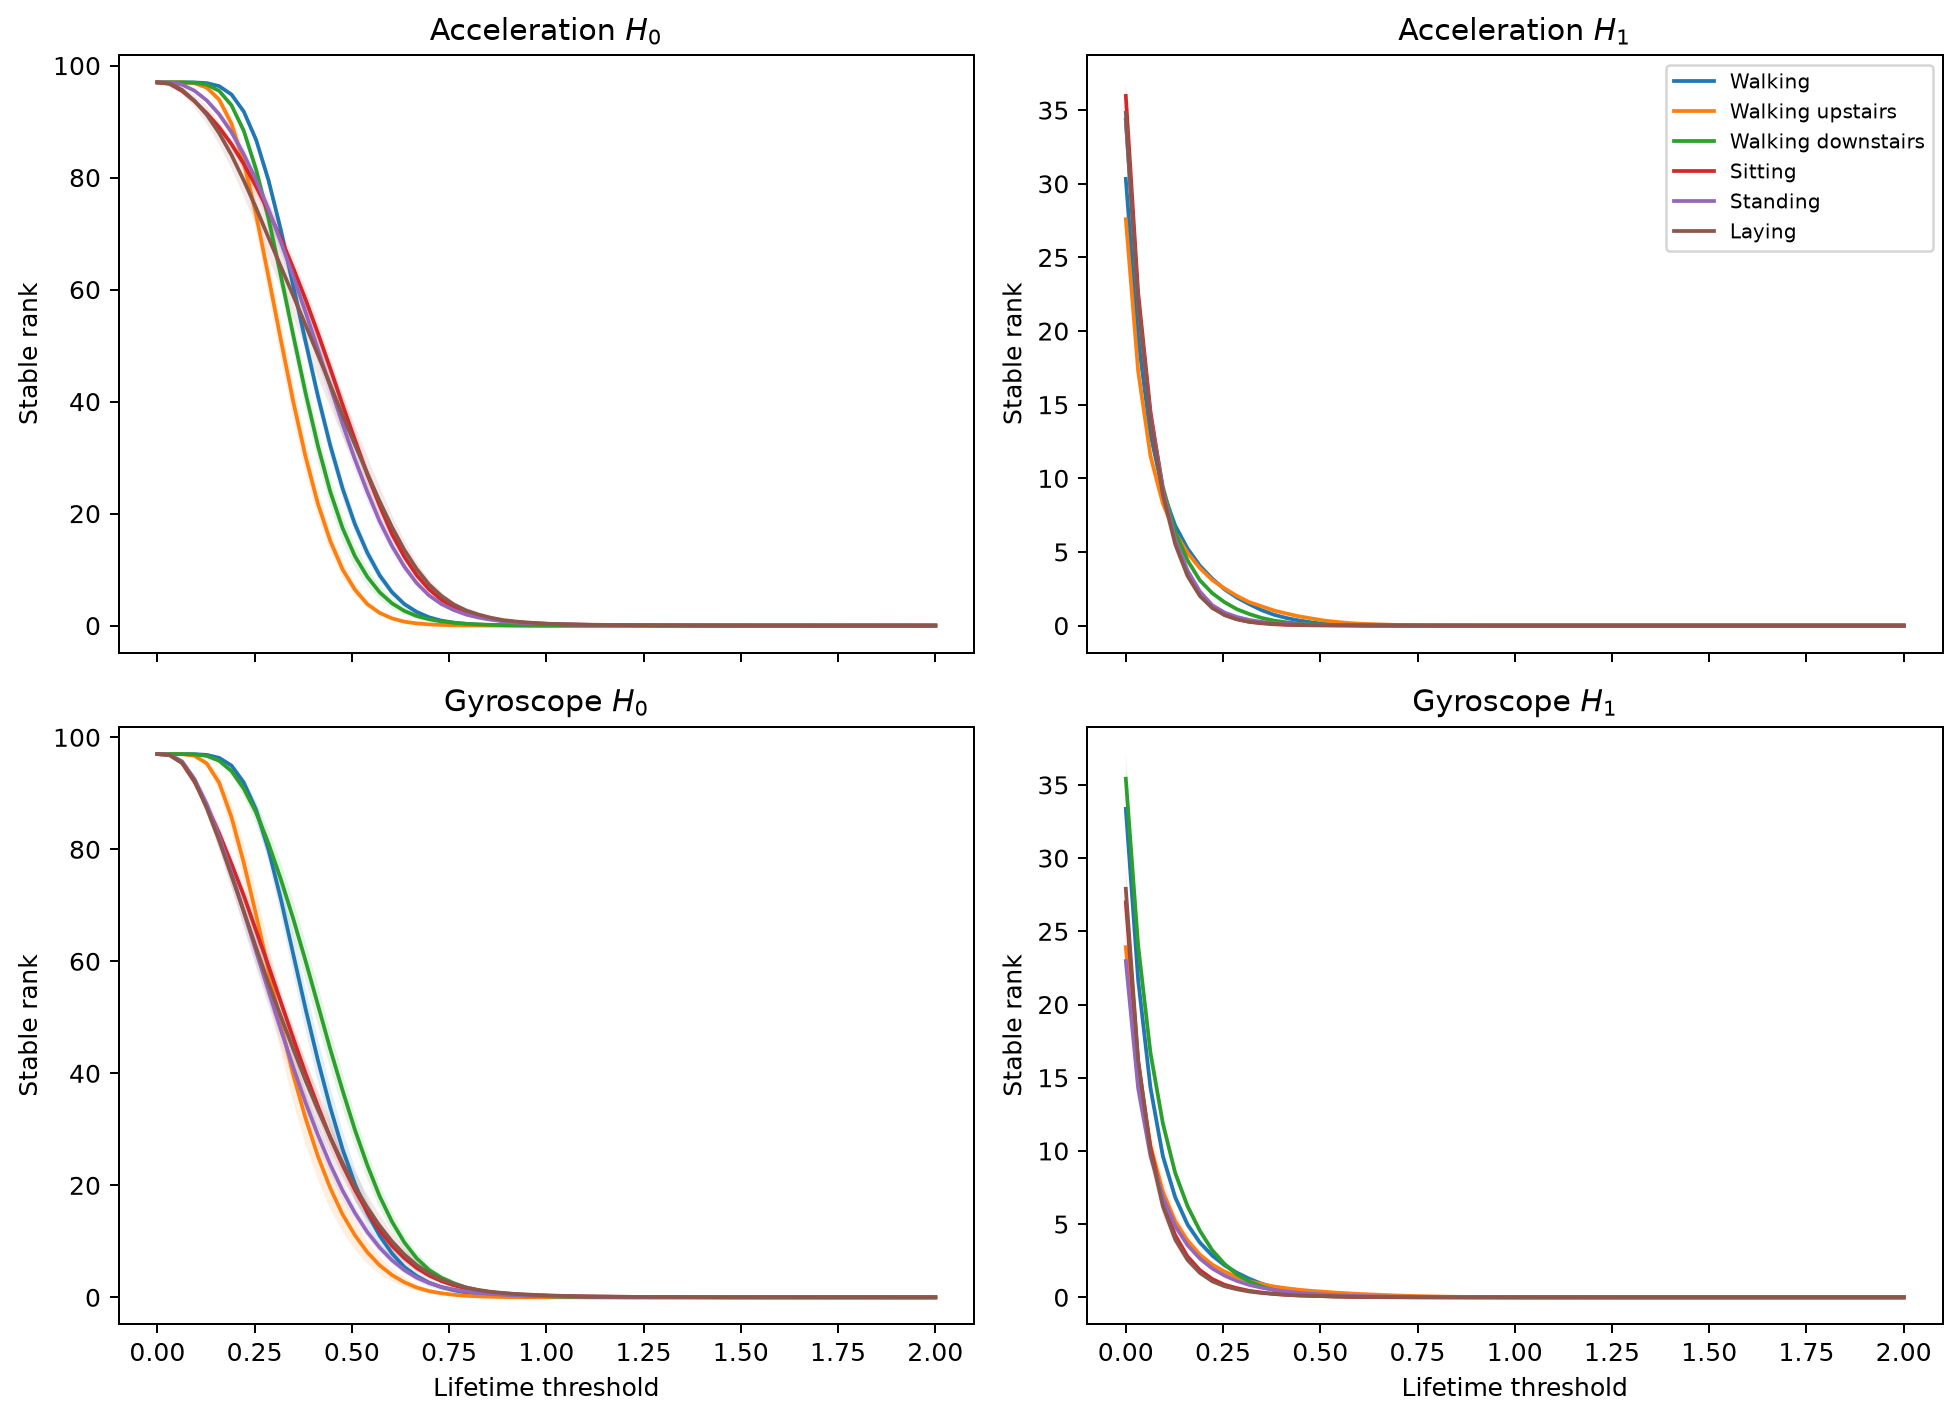
\includegraphics[width=0.95\textwidth]{stable_rank_means.png}
\caption{Subject-balanced stable-rank curves for normalized delay clouds. Windows are first averaged within each of the 21 development subjects; shaded bands show one standard error across those subject means. Curves differ systematically, but several activities remain close.}
\label{fig:ranks}
\end{figure}

\subsection{Diagram summaries and circular coordinates}

Stable ranks retain the distribution of lifetimes but discard birth scales and the identity of individual classes. We therefore construct a second, lower-dimensional view from the same normalized delay clouds. For each sensor, six numbers summarize the diagrams: the mean and final $H_0$ merge scales, the number of finite $H_1$ bars, the longest $H_1$ lifetime, total $H_1$ persistence, and the birth scale of the longest $H_1$ bar.

The longest $H_1$ class is also used to define a circle-valued coordinate following the persistent-cohomology construction of de Silva, Morozov, and Vejdemo-Johansson \cite{circular-coordinates}. Ripser returns a representative persistent cocycle $\alpha$ over $\mathbb F_{47}$. We lift its coefficients to integers and smooth it at the midpoint of its persistence interval by solving
\[
\widehat f
=\operatorname*{arg\,min}_{f}\|\alpha+\delta f\|_2^2,
\qquad
\theta_i=\widehat f_i\bmod 1.
\]
Here $\delta f$ is the difference of the vertex potentials across every edge present at that filtration scale. The value $\theta_i\in\mathbb R/\mathbb Z$ assigns an angle to delay point $i$. Because the points retain their original temporal order, we unwrap $2\pi\theta_i$ and fit
\[
\operatorname{unwrap}(2\pi\theta_i)=\beta_0+\beta_1 i/50+e_i.
\]
The circular frequency is $|\beta_1|/(2\pi)$ Hz and circular linearity is the regression $R^2$. Frequency measures how quickly the inferred phase winds; linearity measures how closely it behaves like steady periodic motion. If a diagram has no finite $H_1$ class, both values are set to zero.

Thus each sensor contributes eight features and the complete representation is
\[
z_w^{\mathrm{dyn}}\in\mathbb R^{16}.
\]
Exactly the same map is applied to every window from all six activities. It does not assume that only walking is periodic: the analysis asks whether the inferred topology and phase differ systematically among walking, stair motion, and the three static postures.

\section{Experimental design}

\subsection{Feature families and controls}

The primary analysis compares seven prespecified representations:

\begin{description}[style=nextline]
\item[Summary statistics] A 66-dimensional conventional baseline containing axis-wise mean, standard deviation, extrema, median, quartiles, RMS, mean absolute derivative, within-sensor axis correlations, and magnitude summaries.
\item[UCI 561 baseline] The supplied time- and frequency-domain feature vector, including jerk, spectral, entropy, autoregressive, and correlation information.
\item[Instantaneous TDA] Stable ranks of $X_w^{1,1}=\{a_w(i)\}$, which treats samples as an unordered point cloud.
\item[Delay TDA] The primary normalized $m=3,\ell=15$ stable-rank representation.
\item[Delay TDA + scale] Delay TDA plus $s(X)$ for acceleration and gyroscope, exposing the contribution of amplitude.
\item[Shuffled-delay TDA] The same delay construction after a fixed random permutation of each window's 128 samples. This preserves measured values but destroys temporal order.
\item[Delay TDA + statistics] Concatenation of normalized stable ranks and the 66 conventional summaries.
\end{description}

The post-hoc circular-coordinate branch compares four further representations under the same classifier and subject-wise protocol:

\begin{description}[style=nextline]
\item[Diagram summaries] The 12 non-phase diagram summaries, six per sensor.
\item[Circular phase] Frequency and linearity for acceleration and gyroscope, giving four coordinates.
\item[Topological dynamics] All 16 diagram and circular-coordinate features in $z_w^{\mathrm{dyn}}$.
\item[Delay TDA + topological dynamics] The 256 stable-rank samples concatenated with $z_w^{\mathrm{dyn}}$.
\end{description}

To check whether the circular rate has a signal-level interpretation, it is compared with the dominant nonzero fast-Fourier-transform frequency of each window. Spearman correlations are reported separately for dynamic and static activities. This is a validation of association, not an assertion that the topological phase rate and spectral peak must be numerically equal.

The unordered representation has an exact negative control. If $P$ permutes the rows of a window matrix $A$, its pairwise distance matrix becomes $PDP^\mathsf T$. The filtration changes only by a relabeling of vertices; therefore its barcode is unchanged. This equality is verified numerically in the test suite.

Complete time reversal gives a second exact invariance for the delay representation. Reversing a window reverses the order of the $m$ three-coordinate blocks in every delay vector and relabels the 98 points. This is a Euclidean isometry, so the persistence diagrams are unchanged. Delay persistence can therefore encode temporal adjacency and recurrent shape, but not the arrow of time.

The joint representation has a targeted control. Let $\pi$ be a seeded derangement of the 98 delay-point indices and replace it by
\[
q_i^{\mathrm{broken}}=
\left(\sqrt{\lambda}\,\widetilde\Phi_i^a,
\sqrt{1-\lambda}\,\widetilde\Phi_{\pi(i)}^g\right).
\]
The acceleration cloud is unchanged and the gyroscope cloud is merely row-permuted. Their marginal distances and separate persistence diagrams are therefore exactly preserved; only their cross-sensor pairing changes. Seed 2956 is used for the paired subject comparison, while four further seeds test sensitivity to the arbitrary derangement. The marginal-set equality is verified in the test suite.

\subsection{Classification and validation}

Every feature set uses the same pipeline: coordinate-wise standardization followed by a class-weighted radial-basis SVM \cite{scikit-learn}. Hyperparameters are selected among
\[
C\in\{0.1,1,10\},\qquad
\gamma\in\{\text{scale},0.001,0.01\}
\]
using nested subject-wise validation. Five outer stratified group folds estimate development performance. Within each outer training portion, four further stratified group folds select $C$ and $\gamma$; the held-out outer subjects play no role in that choice. A separate five-fold search on all 21 development subjects selects the model fitted before prediction on the nine official test subjects. The primary score is balanced accuracy; macro-$F_1$ is secondary. A 95\% interval is obtained by bootstrapping subjects, not individual overlapping windows, 2,000 times. For the two paired topological comparisons, we also enumerate all $2^9$ sign assignments of the nine subject-level differences. This gives an exact two-sided test under the null that the paired signs are exchangeable.

The test split is used for one confirmatory evaluation round. Sensitivity to $(m,\ell)$ and metric is assessed only by grouped cross-validation on the development subjects with frozen classifier settings. After opening the test results, we perform explicitly post-hoc extensions inspired by earlier course projects: sensor and homology ablations, nearest-prototype classification with $d_{[0,2]}$, hierarchical clustering, a subject-wise label-permutation null, circular-coordinate dynamics, and the Euclidean and max-product acceleration--gyroscope constructions. The circular-coordinate models repeat the full nested grouped selection before the official test is reported; because the branch was designed after seeing the primary result, its test scores remain exploratory rather than a second confirmatory evaluation.

\section{Results}

\subsection{Subject-independent classification}

\begin{table}[H]
\centering
\caption{Balanced accuracy under nested subject-wise development folds and on the official subject-disjoint test split. Intervals bootstrap the nine test subjects.}
\label{tab:models}
\begin{tabular}{lccc}
\toprule
Representation & Nested CV & Official test & Test 95\% CI \\
\midrule
Summary statistics & 0.824 & 0.852 & [0.811, 0.886] \\
UCI 561 baseline & 0.935 & 0.954 & [0.932, 0.974] \\
Instantaneous TDA & 0.520 & 0.558 & [0.516, 0.603] \\
Delay TDA & 0.529 & 0.580 & [0.548, 0.615] \\
Delay TDA + scale & 0.618 & 0.640 & [0.614, 0.671] \\
Shuffled-delay TDA & 0.481 & 0.503 & [0.467, 0.538] \\
Delay TDA + statistics & 0.785 & 0.794 & [0.741, 0.837] \\
\bottomrule
\end{tabular}
\end{table}

\begin{figure}[H]
\centering
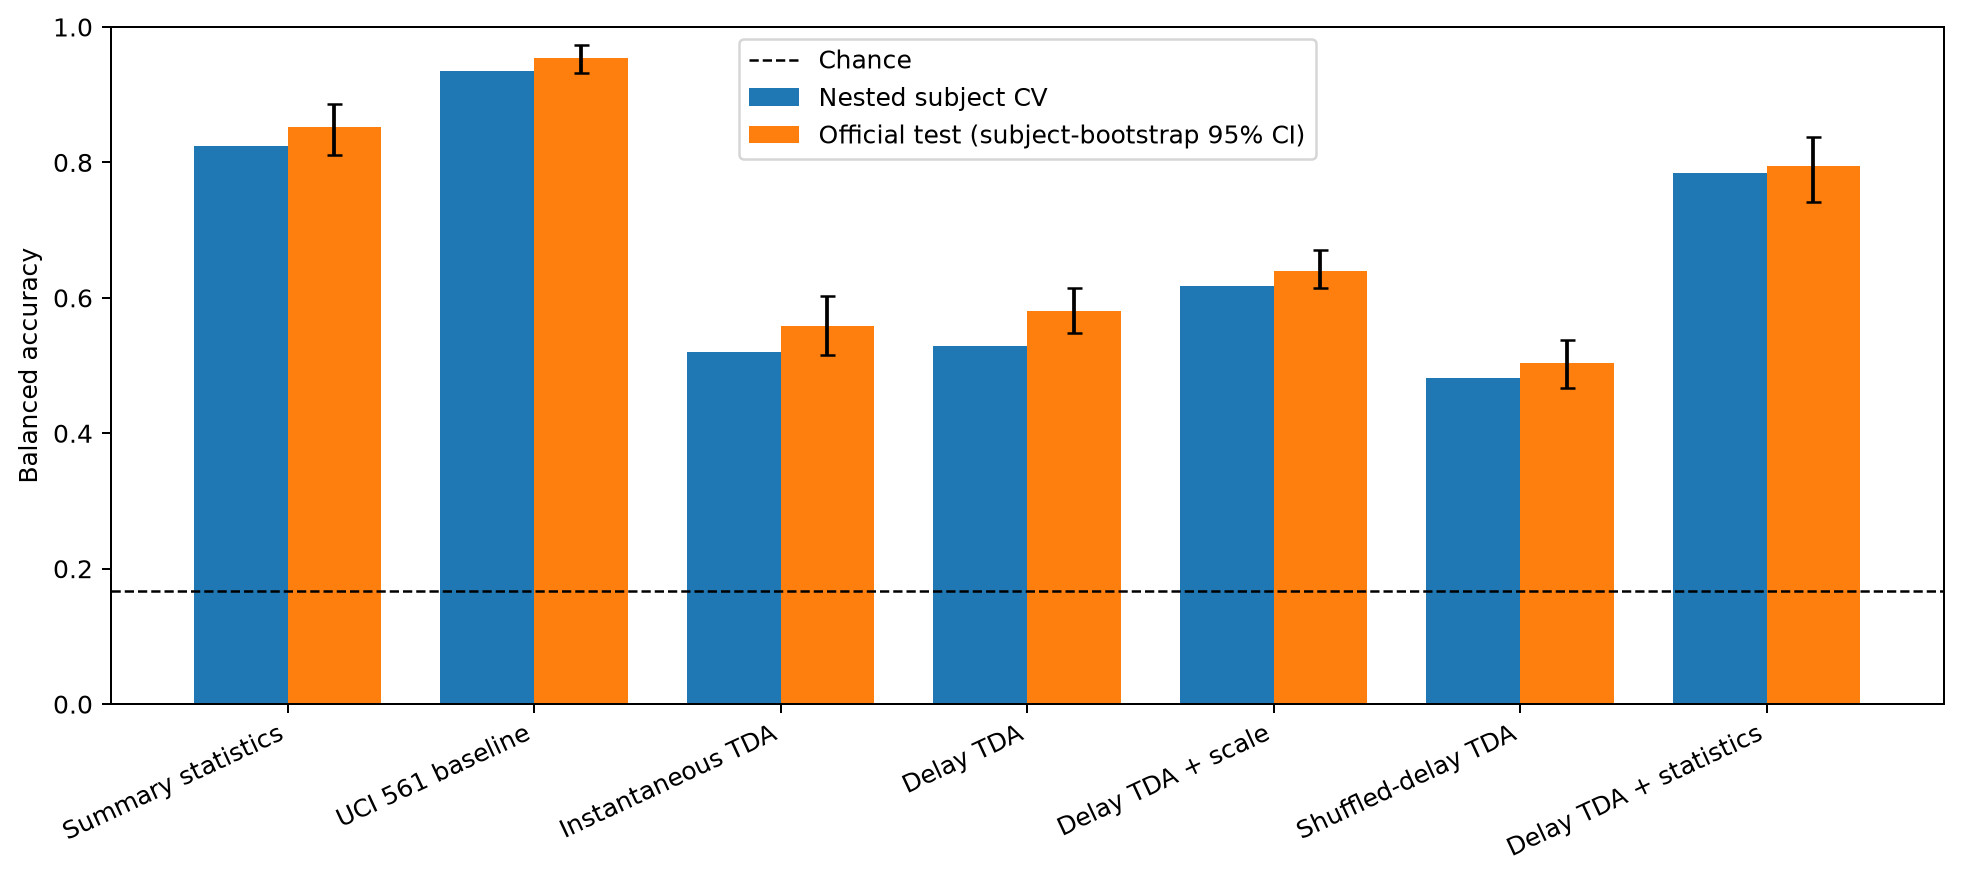
\includegraphics[width=\textwidth]{model_comparison.png}
\caption{Nested development validation and the official test give the same broad ordering. Error bars are subject-bootstrap 95\% intervals for the official test; chance balanced accuracy is $1/6$.}
\label{fig:models}
\end{figure}

Delay TDA exceeds the unordered representation by 0.022 on the test subjects, but the paired subject-bootstrap interval $[-0.001,0.043]$ includes zero and the sign-flip value is $p=0.125$. Against the shuffled control, the difference is 0.075 with interval $[0.037,0.108]$ and $p=0.0117$, positive for eight of nine subjects. Temporal adjacency matters, although the delay-versus-instantaneous comparison is inconclusive.

Adding only two cloud-scale values raises performance by 0.059, confirming that motion magnitude contains information removed by normalization. Conventional summaries remain substantially stronger. Concatenating topological and statistical features reduces rather than improves test performance, so the experiment gives no evidence that this topological vectorization adds predictive value.

\begin{figure}[H]
\centering
\begin{subfigure}{0.49\textwidth}
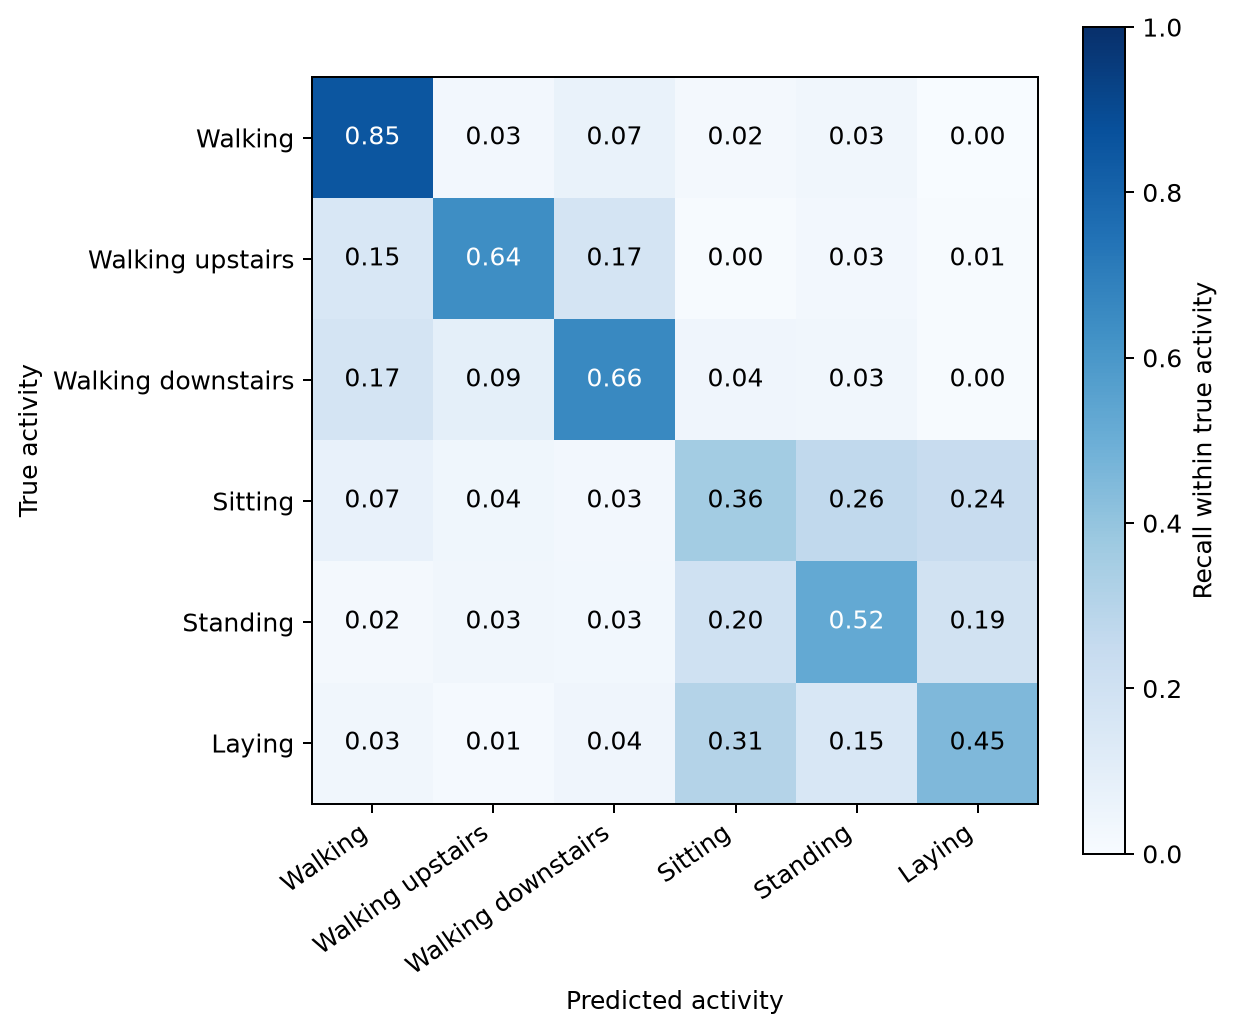
\includegraphics[width=\textwidth]{confusion_delay_tda.png}
\caption{Normalized delay TDA.}
\end{subfigure}
\hfill
\begin{subfigure}{0.49\textwidth}
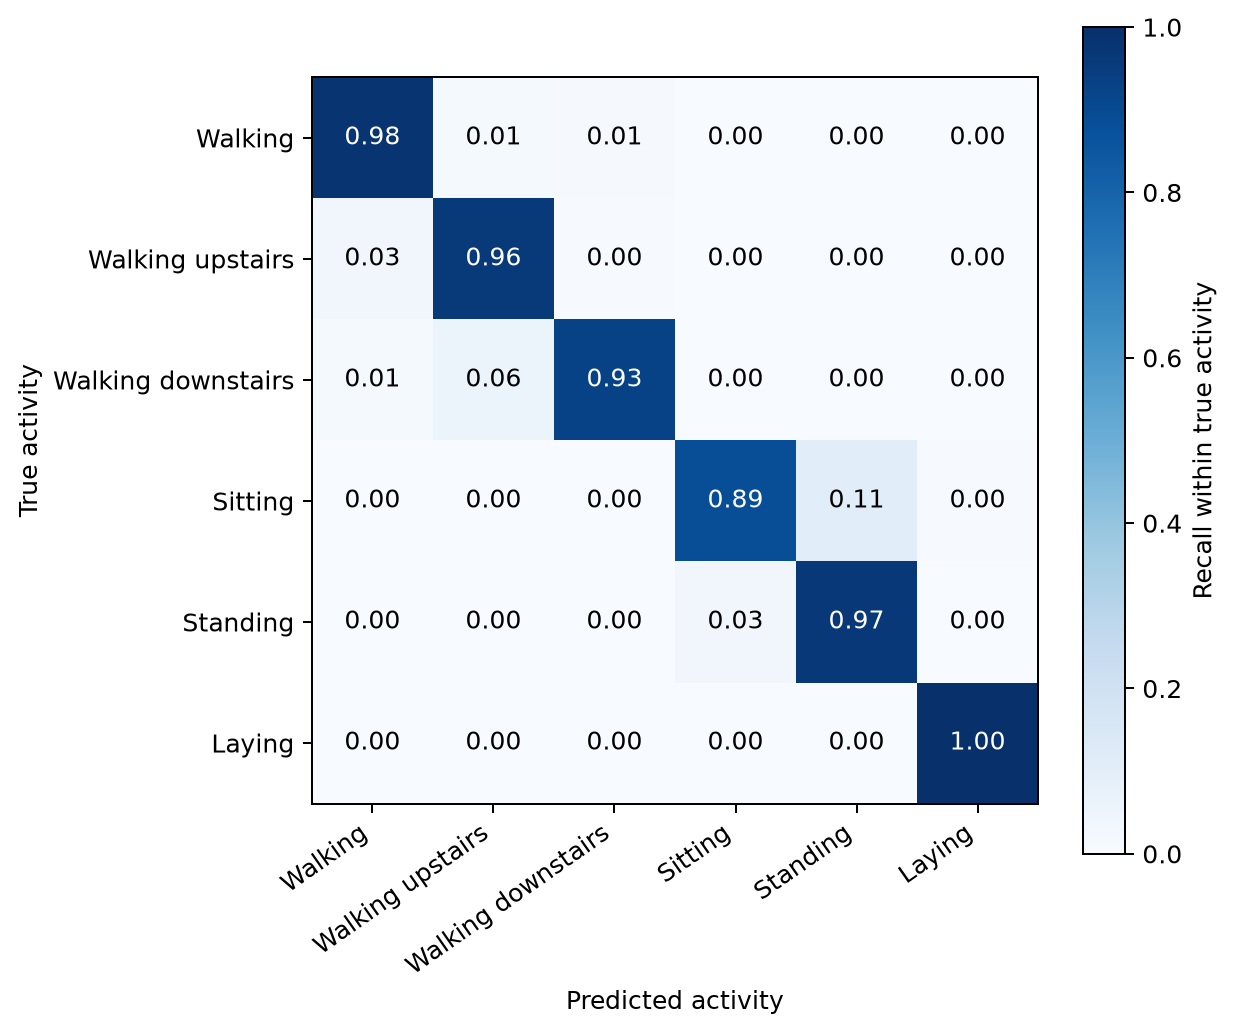
\includegraphics[width=\textwidth]{confusion_uci_baseline.png}
\caption{Supplied UCI 561 features.}
\end{subfigure}
\caption{Row-normalized confusion matrices on the official test subjects. Delay topology identifies walking most reliably but confuses the three static postures.}
\label{fig:confusion}
\end{figure}

\subsection{Stable-rank geometry across subjects}

For every development subject and activity, we average the window-level stable-rank vectors. We then compute $d_{[0,2]}$ on the common threshold grid. The mean distance between different activities and different subjects is 18.93, compared with 13.75 for the same activity across different subjects, a ratio of 1.38.

\begin{figure}[H]
\centering
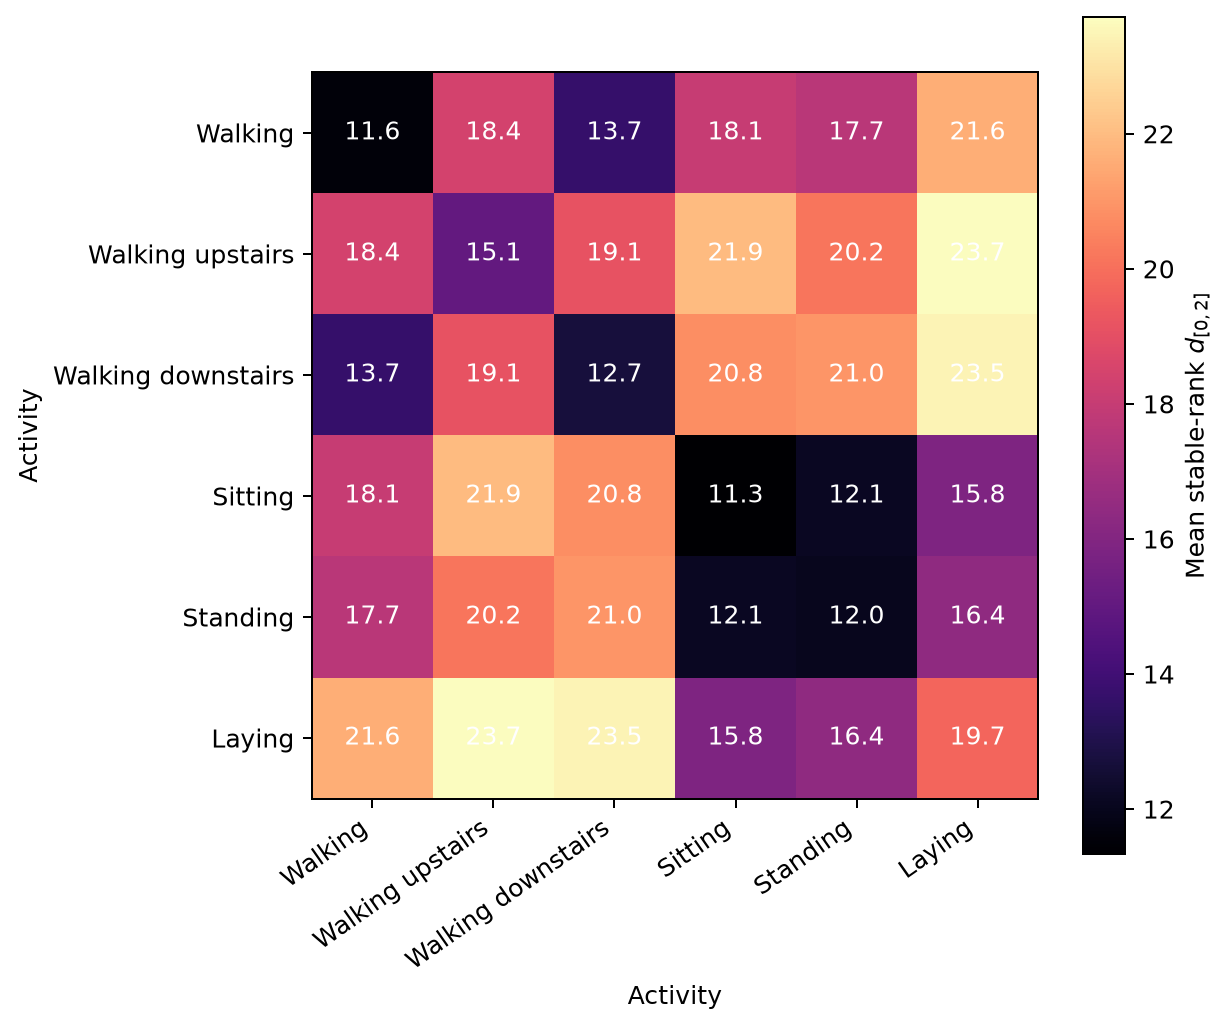
\includegraphics[width=0.76\textwidth]{activity_stable_rank_distances.png}
\caption{Mean $d_{[0,2]}$ distance between subject-activity stable-rank prototypes. Diagonal entries compare the same activity across different subjects. Walking and walking downstairs, and sitting and standing, are particularly close.}
\label{fig:distances}
\end{figure}

Stable ranks separate dynamic and static activities into broad families, while nearby activities within each family overlap. Laying has unusually large within-activity variation (19.73), suggesting subject-specific posture geometry after amplitude removal.

\subsection{Sensitivity and perturbation}

The development-subject balanced accuracy remains between 0.529 and 0.551 across the tested embedding parameters and metrics. Cityblock distance is slightly higher than the primary Euclidean result, but the entire range spans only 0.022. The result is therefore not tied to one convenient $(m,\ell)$ pair.

\begin{figure}[H]
\centering
\begin{subfigure}{0.56\textwidth}
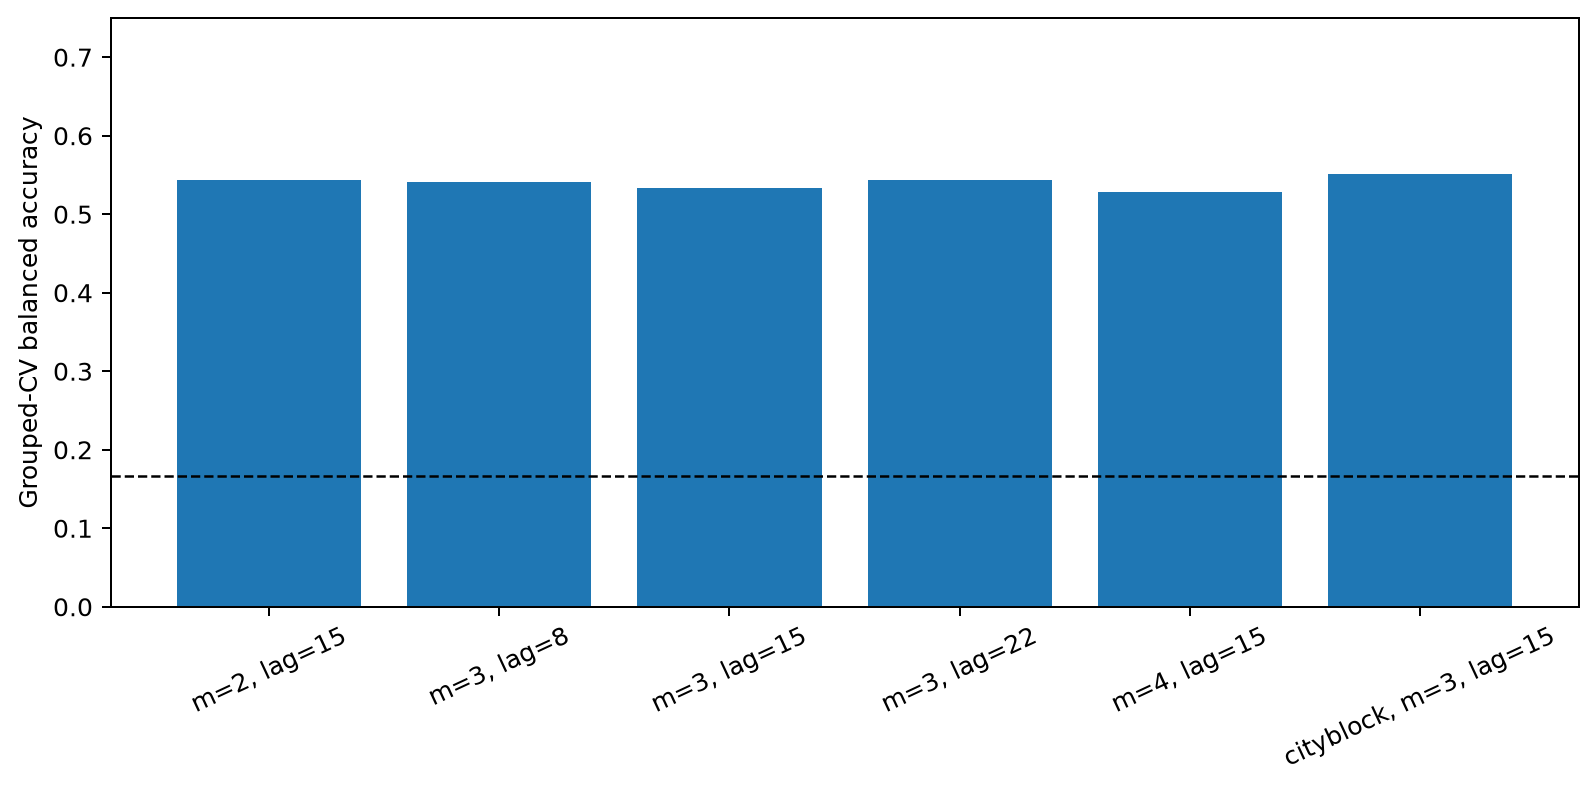
\includegraphics[width=\textwidth]{parameter_sensitivity.png}
\caption{Representation sensitivity.}
\end{subfigure}
\hfill
\begin{subfigure}{0.40\textwidth}
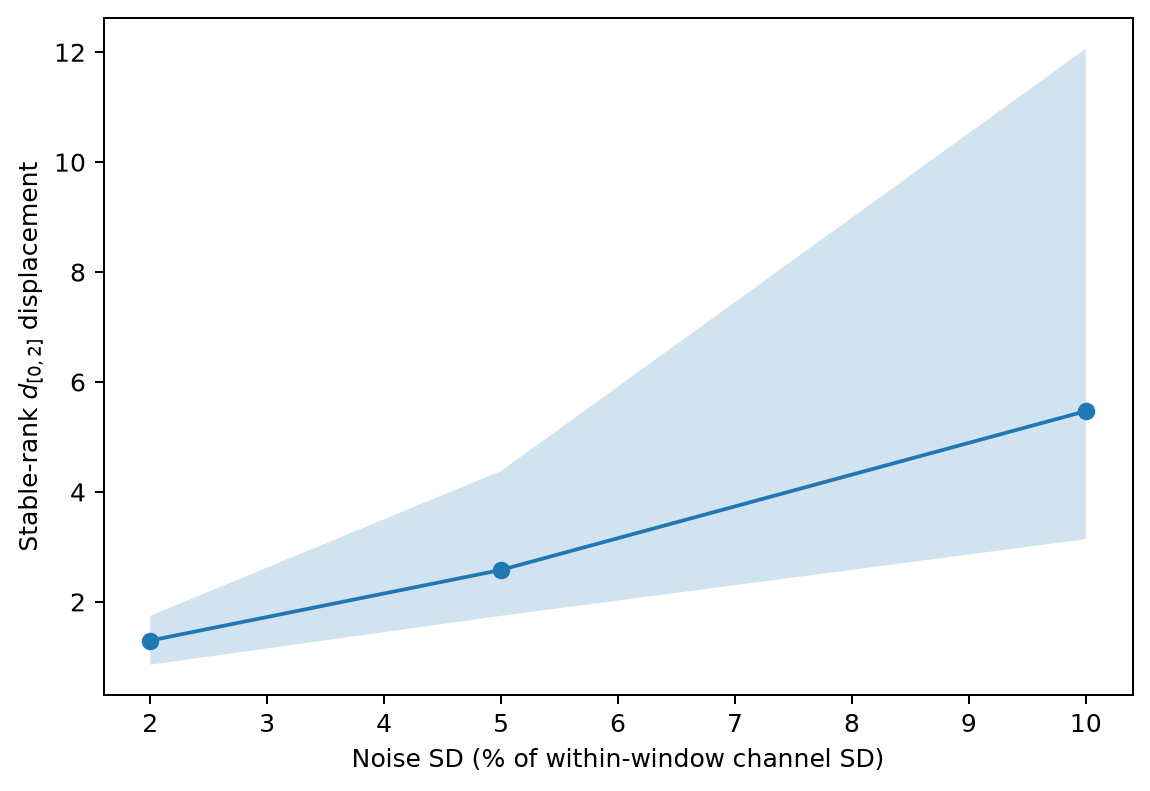
\includegraphics[width=\textwidth]{noise_robustness.png}
\caption{Input-noise perturbation.}
\end{subfigure}
\caption{Robustness analyses use development subjects. Parameter changes leave classification nearly unchanged. Stable-rank displacement increases smoothly with Gaussian noise.}
\label{fig:robustness}
\end{figure}

For the noise experiment, 60 windows per activity are selected. Independent Gaussian noise is added at 2\%, 5\%, and 10\% of each window's channel-wise standard deviation, followed by complete recomputation of normalized delay topology. Mean $d_{[0,2]}$ displacement is 1.30, 2.58, and 5.47 respectively. These equal approximately 9\%, 19\%, and 40\% of the mean same-activity cross-subject distance. The gradual response is consistent with the course's stability mechanism: close Lipschitz maps induce homotopic maps after a scale shift and hence equal maps on homology \cite[Points 197 and 222]{course-notes}. The finite experiment illustrates, but does not prove, a stability theorem.

\subsection{Alternative topological analyses}

The four 64-coordinate blocks show which topological information matters. With the primary frozen SVM settings, acceleration alone reaches 0.470 balanced accuracy and gyroscope alone 0.374. Combining both sensors gives 0.442 from $H_0$ alone and 0.451 from $H_1$ alone, while all four blocks give 0.533. Both sensors and both homology degrees contribute.

We also classify directly with the stable-rank distance. Each subject-activity pair is represented by its mean stable rank, and a query is assigned to the nearest activity prototype in $d_{[0,2]}$. This rule reaches 0.351 grouped-CV balanced accuracy at window level and 0.476 at subject-activity level.

For a structural null test, the six activity names are independently permuted within each subject. This preserves one prototype per activity and all subject effects but destroys label correspondence across people. Across 2,000 permutations the mean score is 0.168 and the 95\% null interval is $[0.095,0.246]$. None reaches the observed 0.476, giving $p=(0+1)/(2000+1)=0.0005$.

\begin{figure}[H]
\centering
\begin{subfigure}{0.80\textwidth}
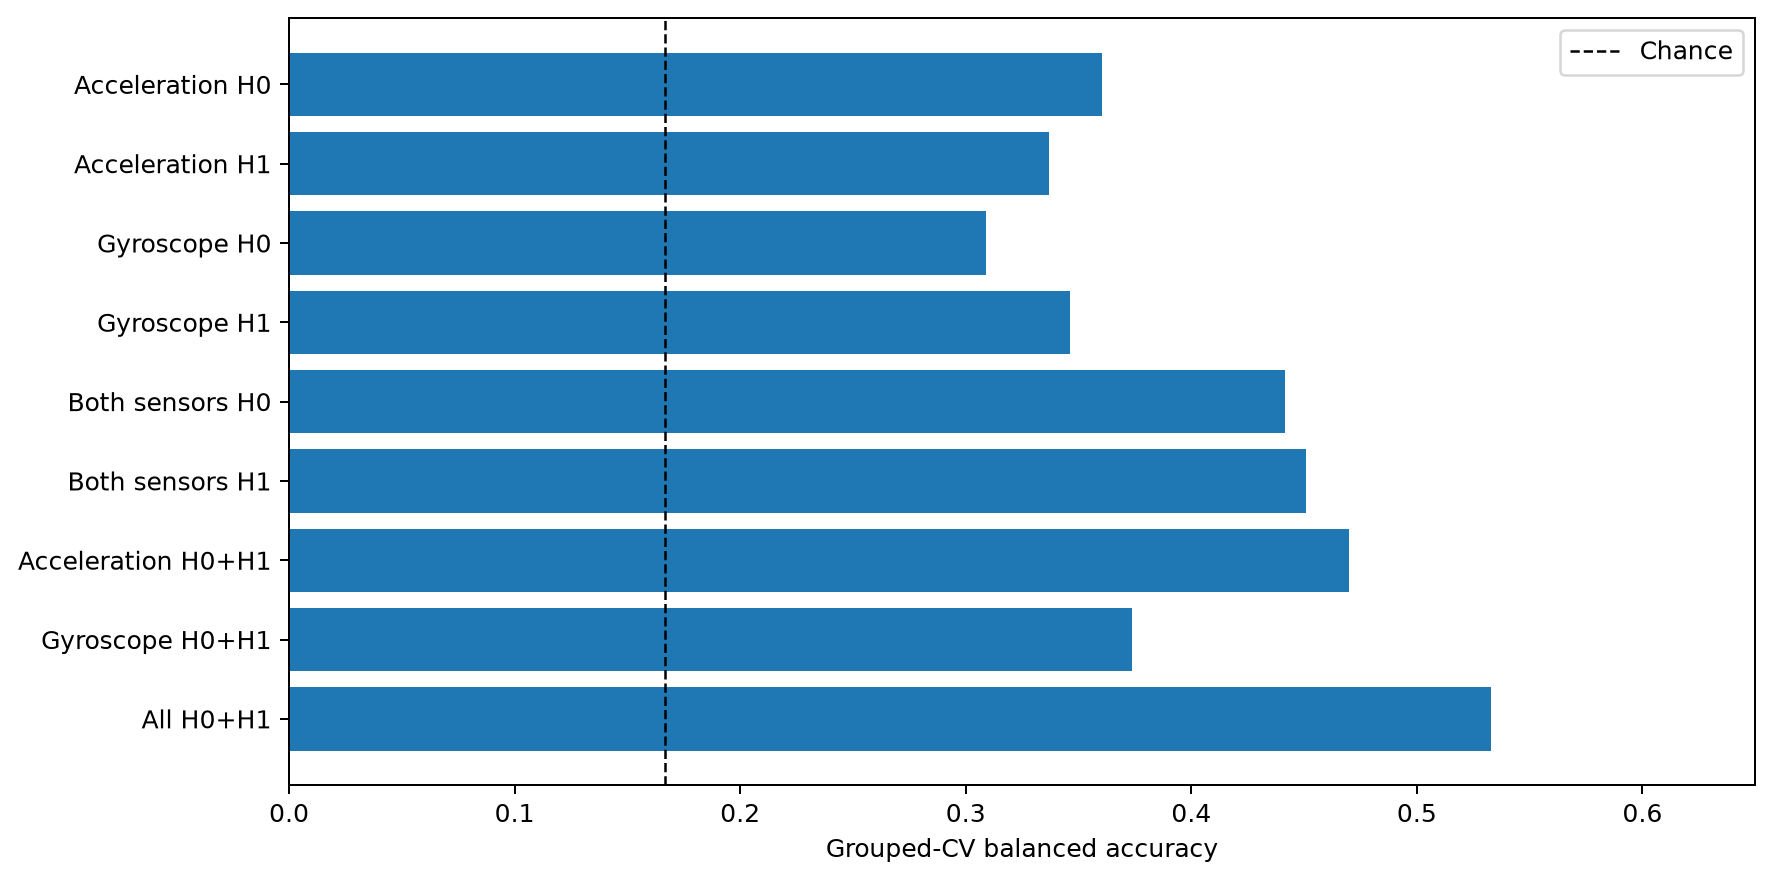
\includegraphics[width=\textwidth]{topology_ablation.png}
\caption{Sensor and homology ablations on development subjects.}
\end{subfigure}

\begin{subfigure}{0.49\textwidth}
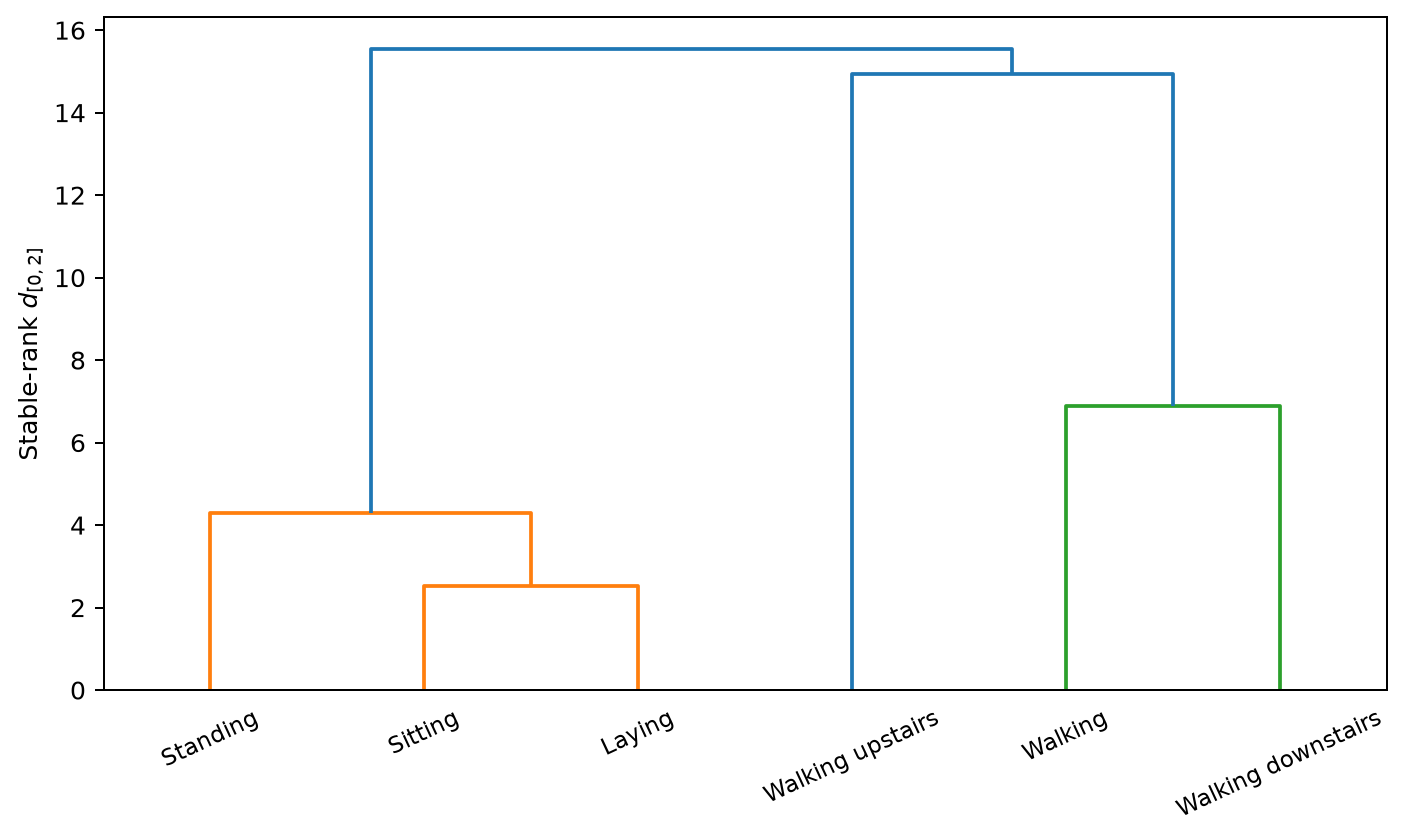
\includegraphics[width=\textwidth]{activity_dendrogram.png}
\caption{Average-linkage clustering in stable-rank $d_{[0,2]}$.}
\end{subfigure}
\hfill
\begin{subfigure}{0.49\textwidth}
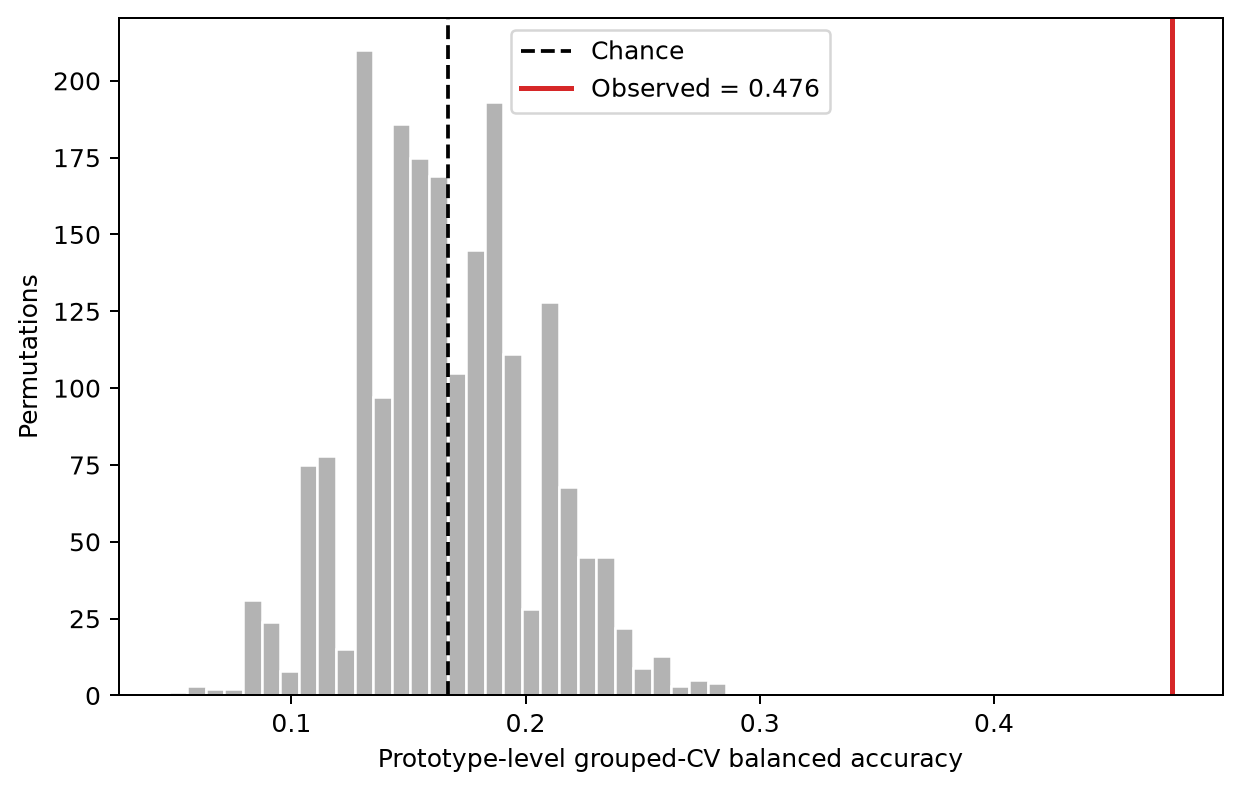
\includegraphics[width=\textwidth]{prototype_permutation_null.png}
\caption{Subject-wise relabeling null.}
\end{subfigure}
\caption{Post-hoc topological diagnostics. The dendrogram recovers a static-activity cluster and a dynamic-activity cluster without using labels in the clustering step; the null distribution shows that the activity correspondence generalizes across subjects.}
\label{fig:extensions}
\end{figure}

The dendrogram gives the same unsupervised split. Sitting, standing, and laying form one cluster. Walking and walking downstairs merge first in a second cluster, followed by walking upstairs.

\subsection{Interpretable topology and circular dynamics}

The 16-feature branch applies the same diagram and circular-coordinate map to every activity. Figure~\ref{fig:dynamics-profiles} shows that it recovers both the dynamic--static division and differences within those groups. After removing each subject's mean, the strongest activity effects are gyroscope circular frequency ($\eta_p^2=0.844$), acceleration circular linearity ($0.787$), acceleration longest $H_1$ lifetime ($0.754$), gyroscope circular linearity ($0.753$), and gyroscope longest $H_1$ lifetime ($0.697$). Thus the result is not based on one walking example: all 21 development subjects and all six labels enter each effect estimate.

\begin{figure}[H]
\centering
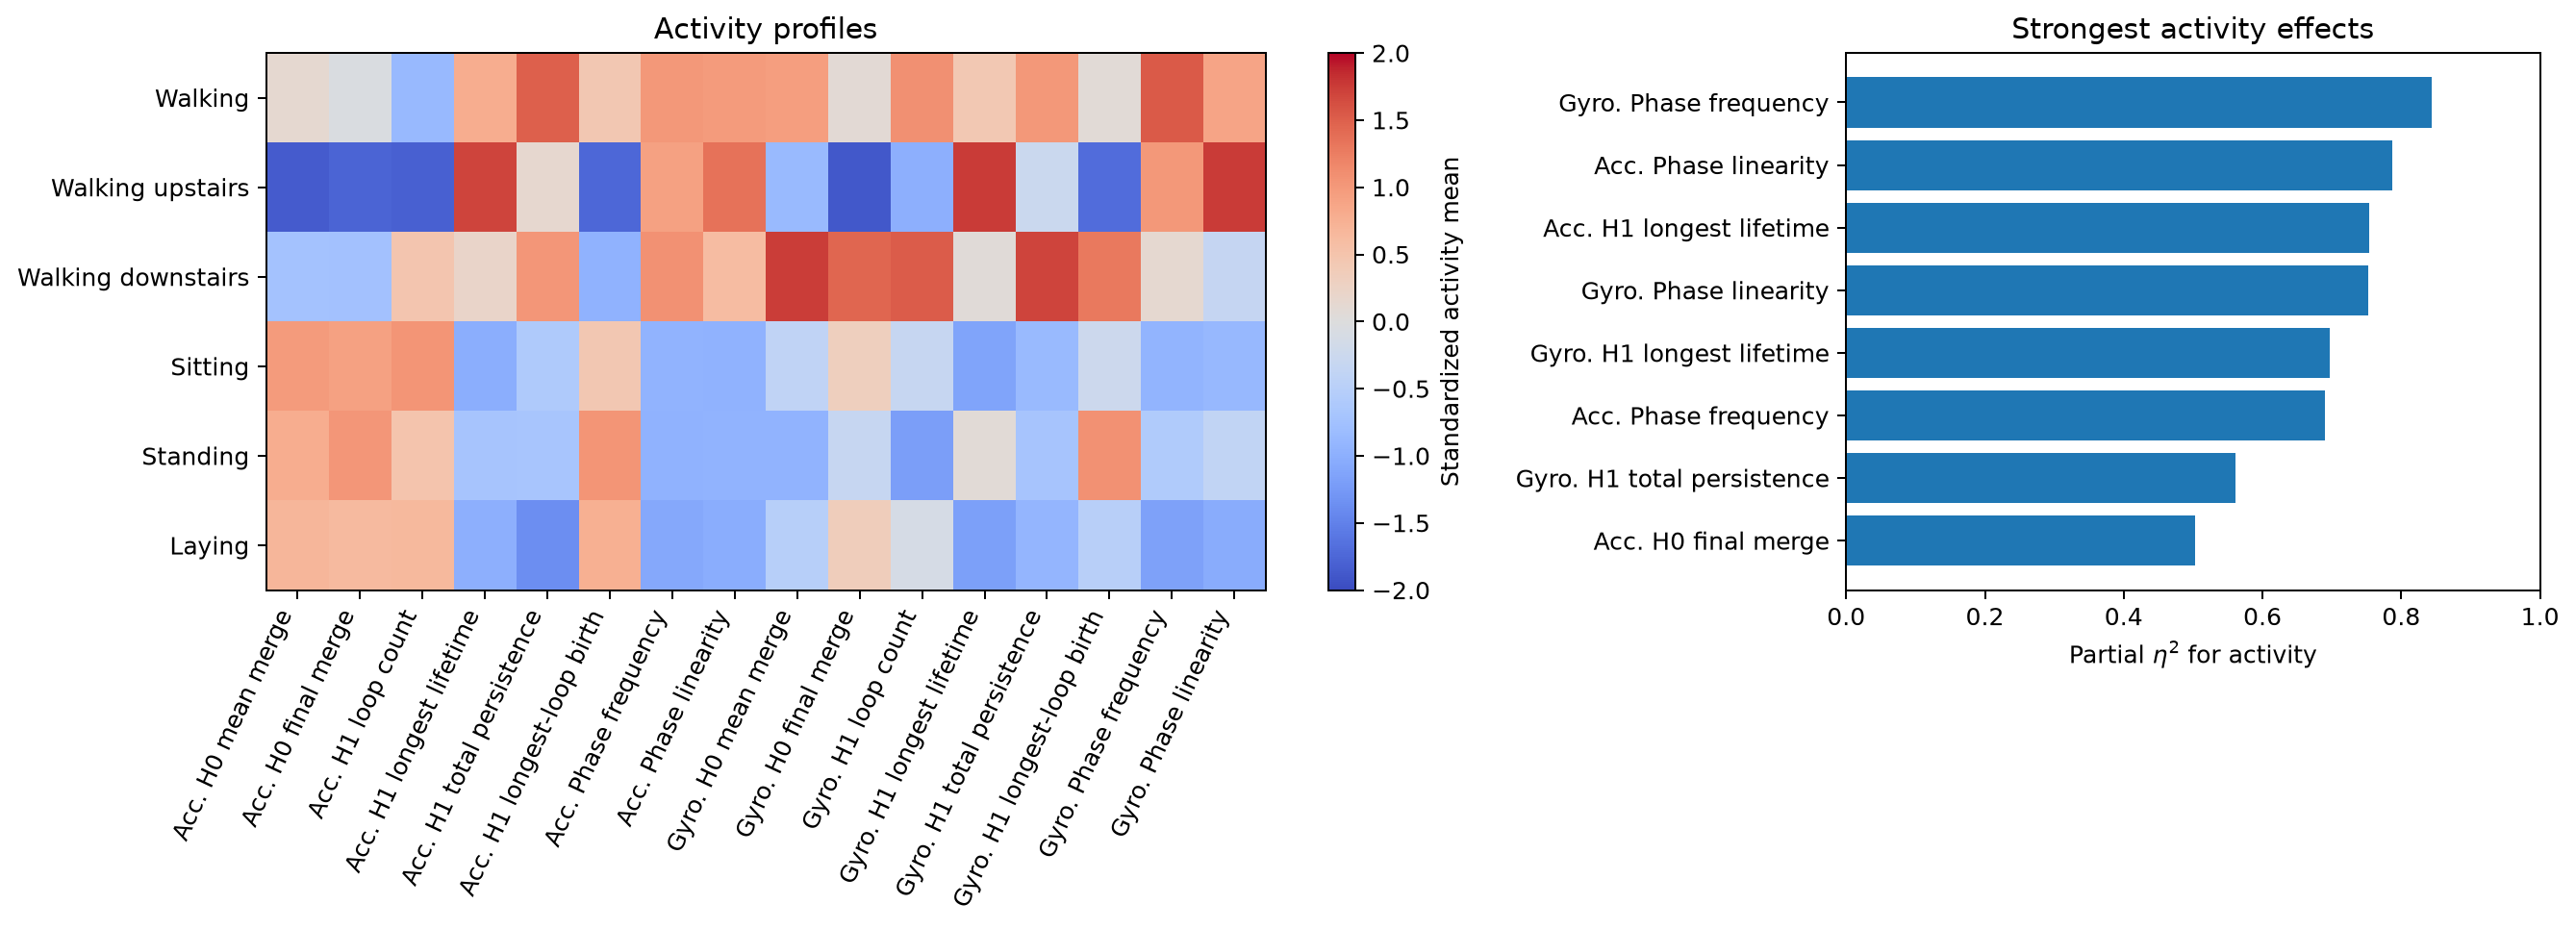
\includegraphics[width=\textwidth]{topological_dynamics.png}
\caption{The same 16 topological-dynamics features across all six activities. Left: subject-balanced activity means, standardized within each feature for display. Right: partial $\eta^2$ for the eight strongest activity effects after removing subject means.}
\label{fig:dynamics-profiles}
\end{figure}

The three dynamic activities have mean acceleration circular frequency 0.898 Hz, compared with 0.408 Hz for the static activities; the gyroscope values are 0.647 and 0.426 Hz. Within the dynamic windows, circular frequency correlates with the ordinary dominant spectral frequency at $\rho=0.362$ for acceleration and $0.271$ for gyroscope. The corresponding acceleration correlation for static windows is only $0.029$. This supports a periodic-motion interpretation, but the circular rate is not the Fourier peak: it follows the phase of one persistent loop and is often close to half the strongest signal harmonic.

\begin{table}[H]
\centering
\caption{Classification from the all-activity topology-and-dynamics branch. The branch is post-hoc; intervals bootstrap the nine official test subjects.}
\label{tab:dynamics-models}
\begin{tabular}{lccc}
\toprule
Representation & Nested CV & Official test & Test 95\% CI \\
\midrule
Diagram summaries (12) & 0.539 & 0.577 & [0.533, 0.624] \\
Circular phase (4) & 0.410 & 0.418 & [0.391, 0.447] \\
Topological dynamics (16) & 0.567 & 0.611 & [0.568, 0.653] \\
Delay TDA + topological dynamics (272) & 0.550 & 0.593 & [0.553, 0.632] \\
\bottomrule
\end{tabular}
\end{table}

\begin{figure}[H]
\centering
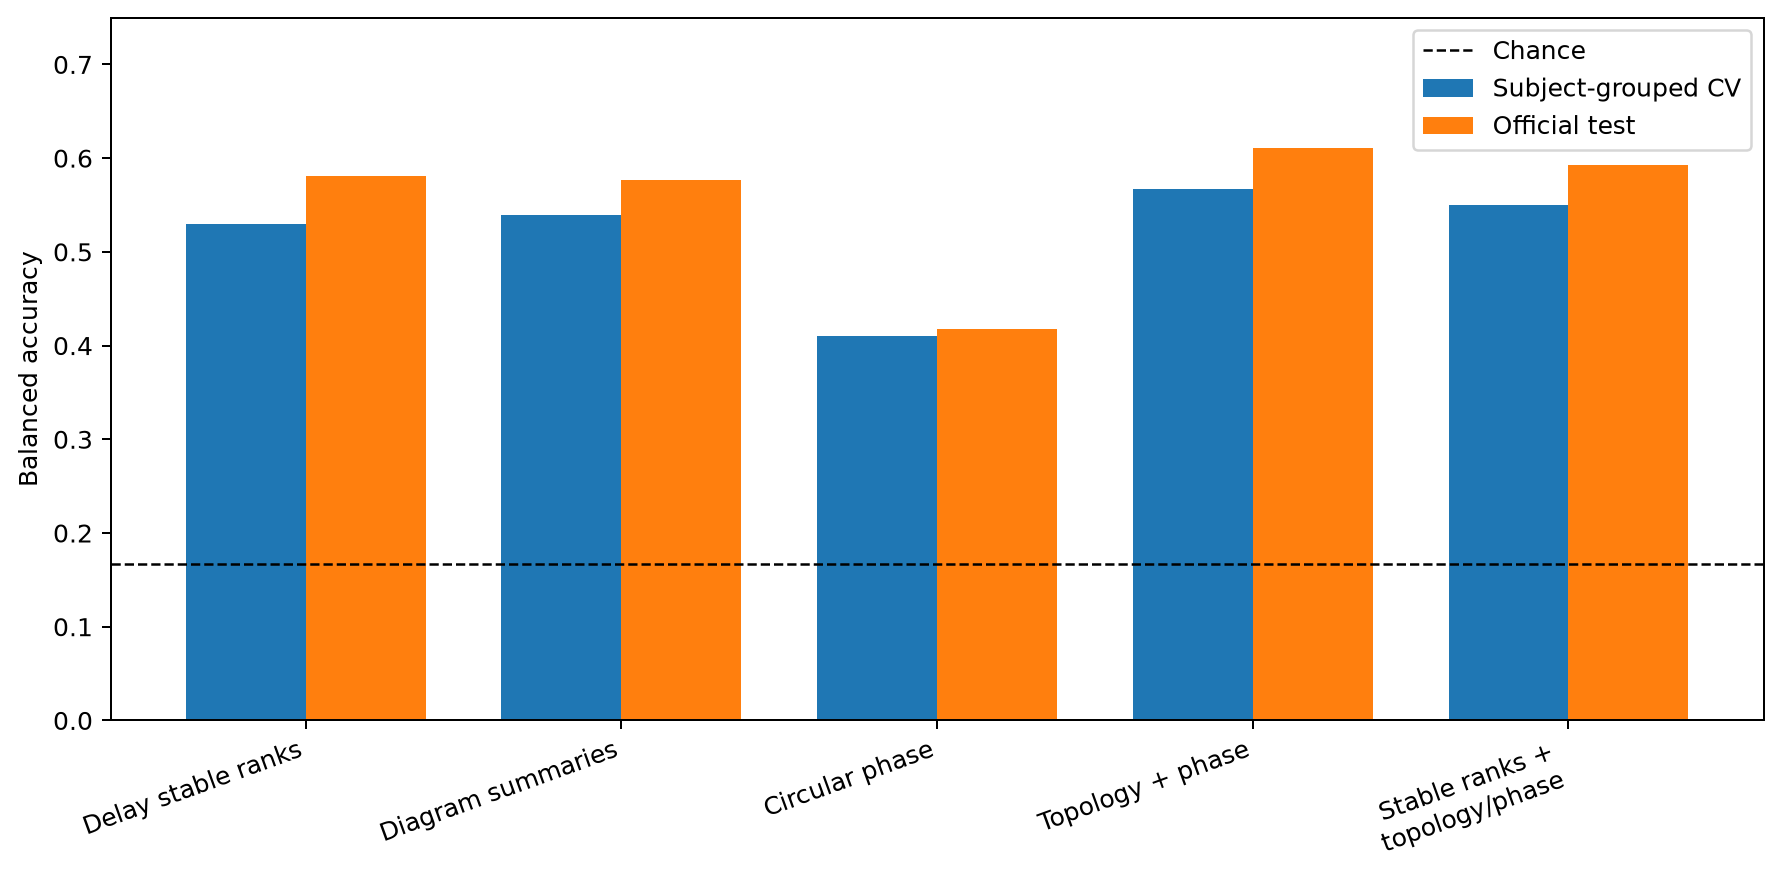
\includegraphics[width=0.90\textwidth]{dynamics_classification.png}
\caption{Grouped development and subject-disjoint test performance for the new branch. Combining diagram summaries with phase is stronger than either part alone; adding the 256 sampled stable ranks does not help further.}
\label{fig:dynamics-classification}
\end{figure}

Topological dynamics improves over the original Delay TDA score from 0.580 to 0.611. The mean paired subject-level difference is 0.031, with bootstrap interval $[0.020,0.040]$, and is positive for eight of nine test subjects. Appending the stable ranks lowers the score to 0.593; combined minus topological dynamics is $-0.018$ with interval $[-0.037,0.000]$. The concise vector therefore captures useful birth, lifetime, and ordered phase information that is blurred or discarded by sampling only the stable-rank curves.

\subsection{Joint acceleration--gyroscope topology}

The separate-sensor representation cannot record whether a particular acceleration fragment occurs simultaneously with a particular gyroscope fragment: it only concatenates two summaries computed independently. The joint cloud changes the metric before persistence is computed. At $\lambda=1/2$, joint topology alone reaches 0.438 balanced accuracy under grouped development validation, compared with 0.533 for separate-sensor topology. However, concatenating the 128 joint coordinates with the 256 separate coordinates reaches 0.560. The mean combined-minus-separate difference over the 21 subject scores is 0.028, with a paired subject-bootstrap 95\% interval of $[0.012,0.044]$.

\begin{figure}[H]
\centering
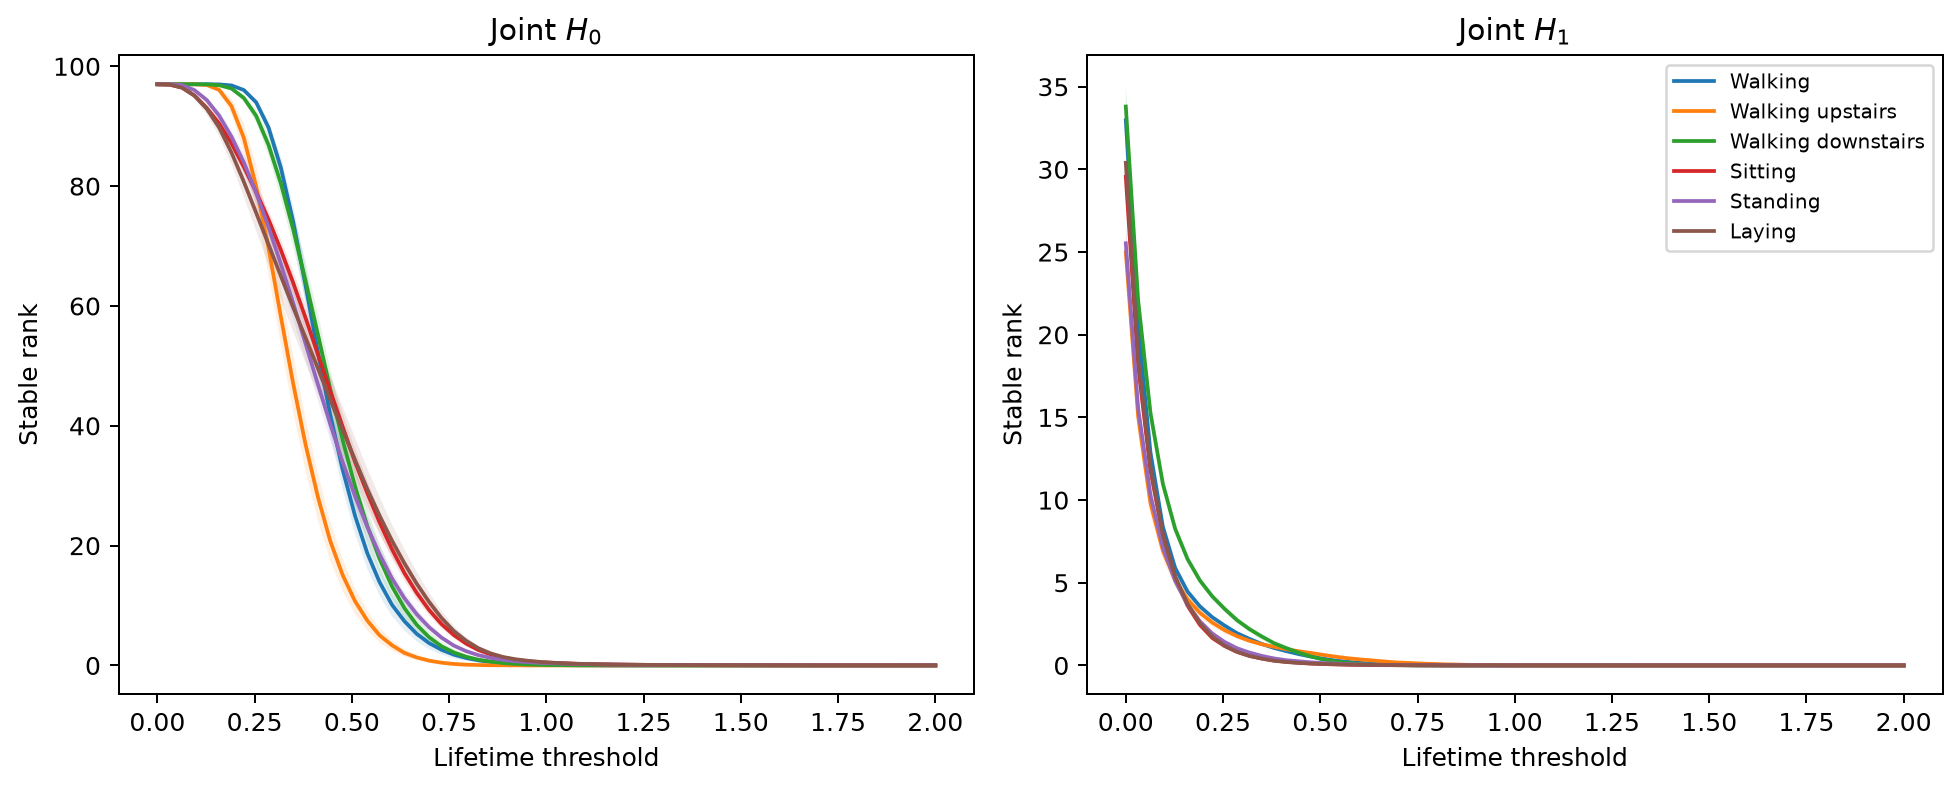
\includegraphics[width=0.90\textwidth]{joint_stable_rank_means.png}
\caption{Subject-balanced stable-rank curves of the equal-weight joint acceleration--gyroscope cloud on the 21 development subjects. The representation contains one $H_0$ and one $H_1$ block rather than separate blocks for each sensor.}
\label{fig:joint-ranks}
\end{figure}

\begin{figure}[H]
\centering
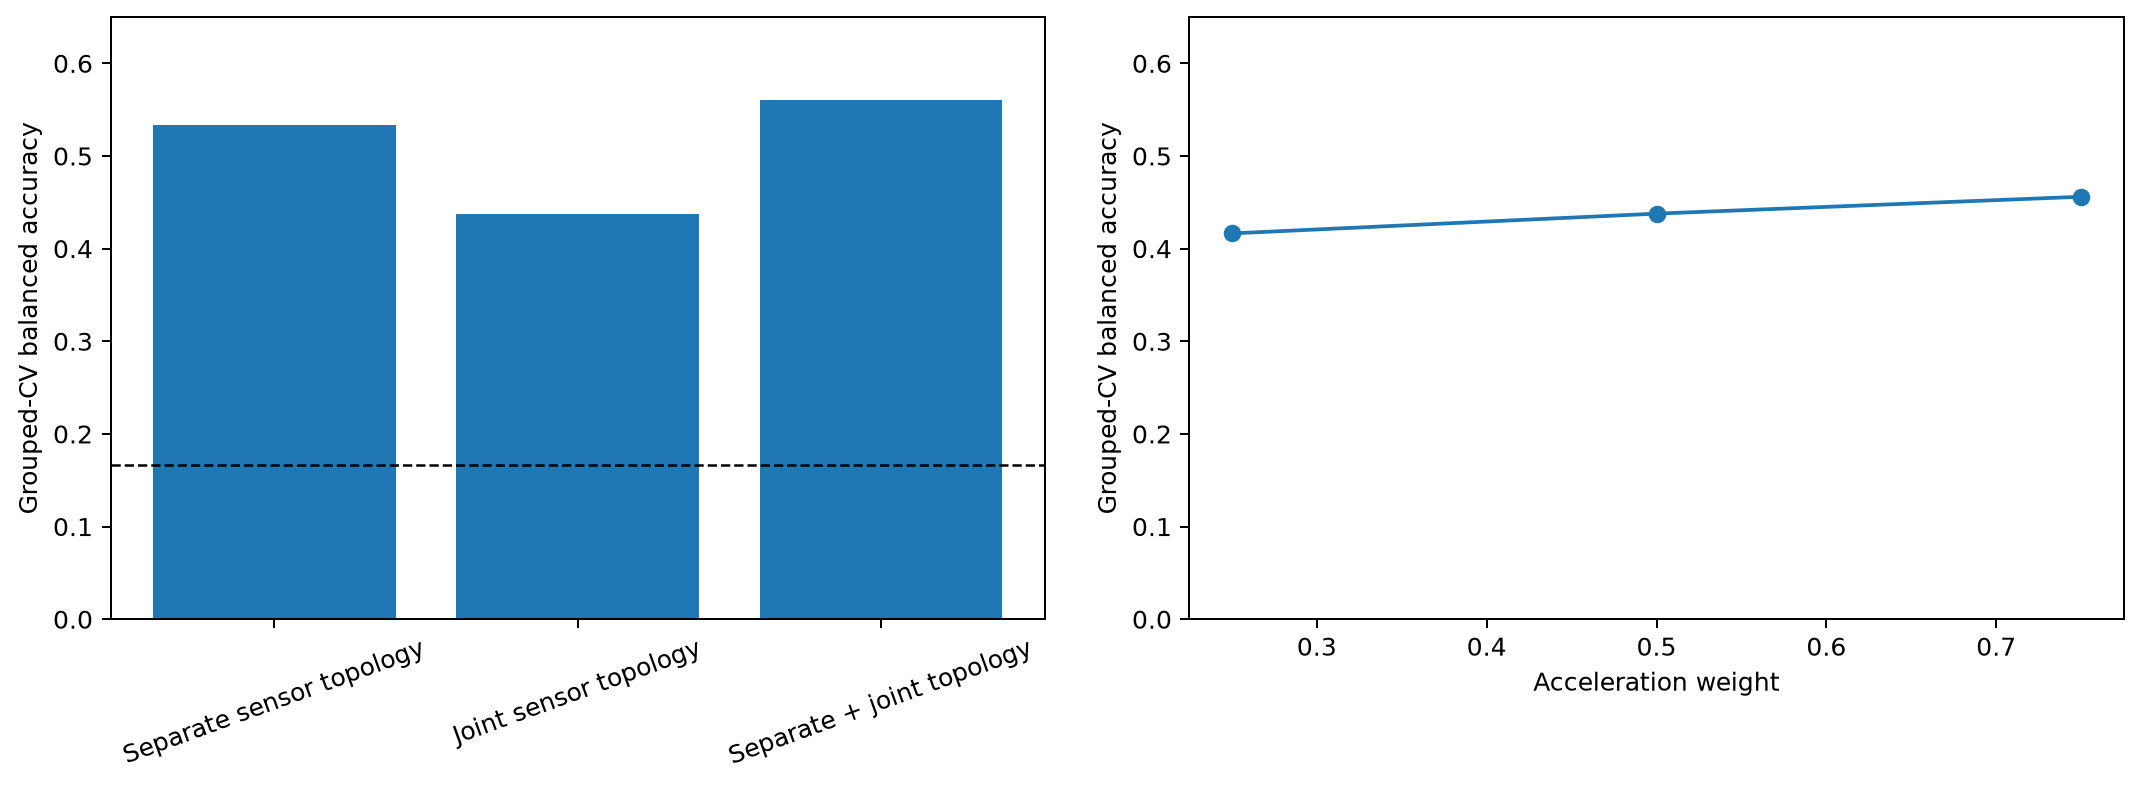
\includegraphics[width=0.86\textwidth]{joint_representation.png}
\caption{Post-hoc grouped development analysis. Joint topology is not a replacement for the separate clouds, but the combined representation improves their mean score. Giving acceleration more weight improves the joint representation, consistent with the sensor ablation.}
\label{fig:joint}
\end{figure}

Within the joint vector, $H_0$ alone scores 0.321 and $H_1$ alone 0.379; together they score 0.438. Acceleration weights 0.25, 0.50, and 0.75 give 0.416, 0.438, and 0.456. The trend agrees with the earlier sensor ablation.

Correctly paired joint topology scores 0.438, while five broken-pairing realizations score 0.417--0.427. For the declared seed, the mean subject-level correct-minus-broken difference is 0.022 with paired bootstrap interval $[-0.006,0.049]$. The point estimate favors synchronization, but the interval includes zero.

\begin{figure}[H]
\centering
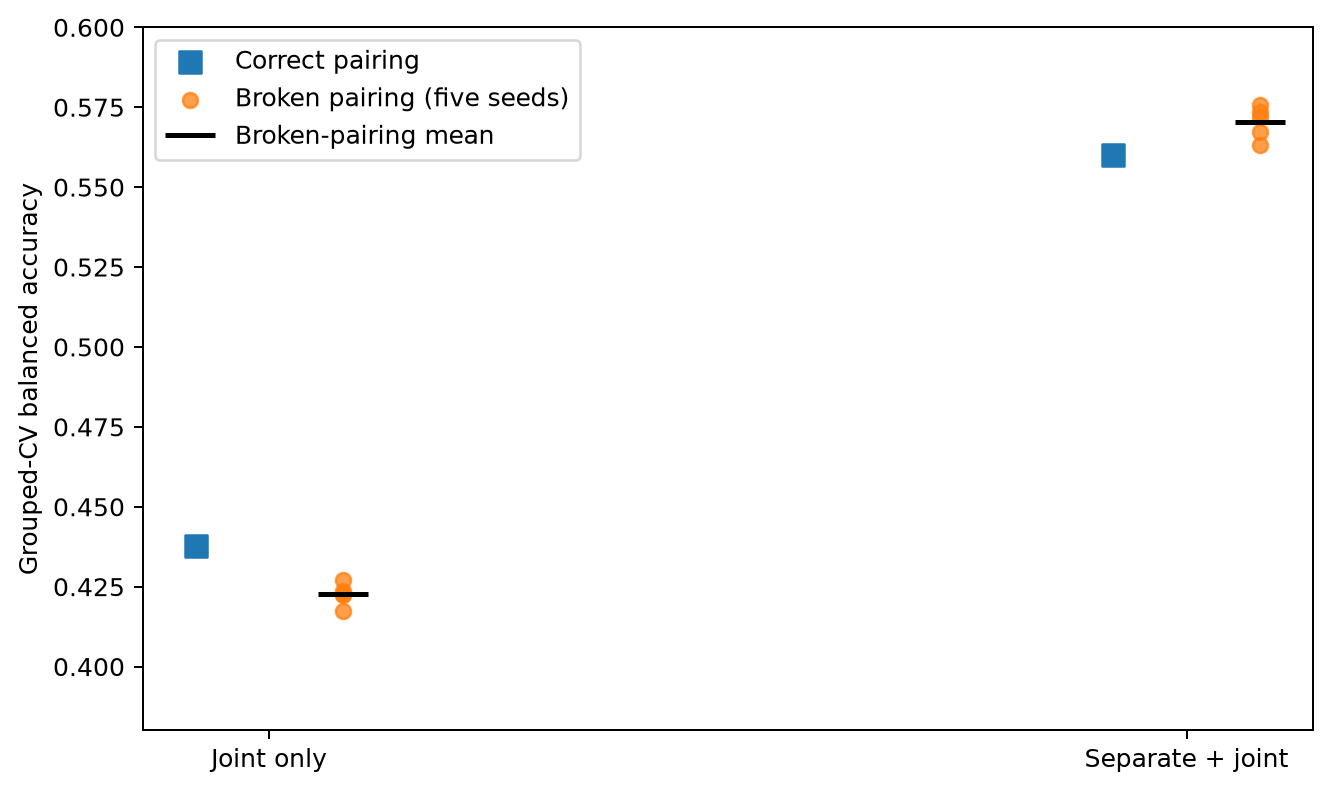
\includegraphics[width=0.74\textwidth]{synchronization_control.png}
\caption{Marginal-preserving synchronization control on the 21 development subjects. Orange points are five seeded derangements and black marks their mean; this across-seed spread is a sensitivity display, not a confidence interval. Correct pairing has no advantage once the joint vector is appended to the separate topology.}
\label{fig:synchronization}
\end{figure}

When appended to separate topology, broken pairing scores 0.563--0.576, compared with 0.560 for correct pairing. For seed 2956, the correct-minus-broken mean is $-0.005$ with interval $[-0.021,0.011]$. Separate plus broken-pairing topology still exceeds separate topology by 0.033 with interval $[0.017,0.048]$. The extra vector helps, but its gain survives removal of the correct sensor alignment. No official test subjects are used in this extension.

\subsection{Max-coupled sensor filtration}

The max-product metric tests a stricter construction: at equal weight, every Vietoris--Rips edge requires simultaneous proximity in both normalized sensor clouds. Max-coupled topology alone reaches 0.425 grouped-CV balanced accuracy, compared with 0.438 for the Euclidean joint cloud and 0.533 for separate-sensor topology. Appending its 128 stable-rank coordinates to the separate 256 coordinates reaches 0.557. The mean combined-minus-separate subject difference is 0.025 with paired bootstrap interval $[0.010,0.039]$.

Acceleration weights 0.25, 0.50, and 0.75 give 0.389, 0.425, and 0.455. As in the Euclidean product, the acceleration-heavy slice performs best.

\begin{figure}[H]
\centering
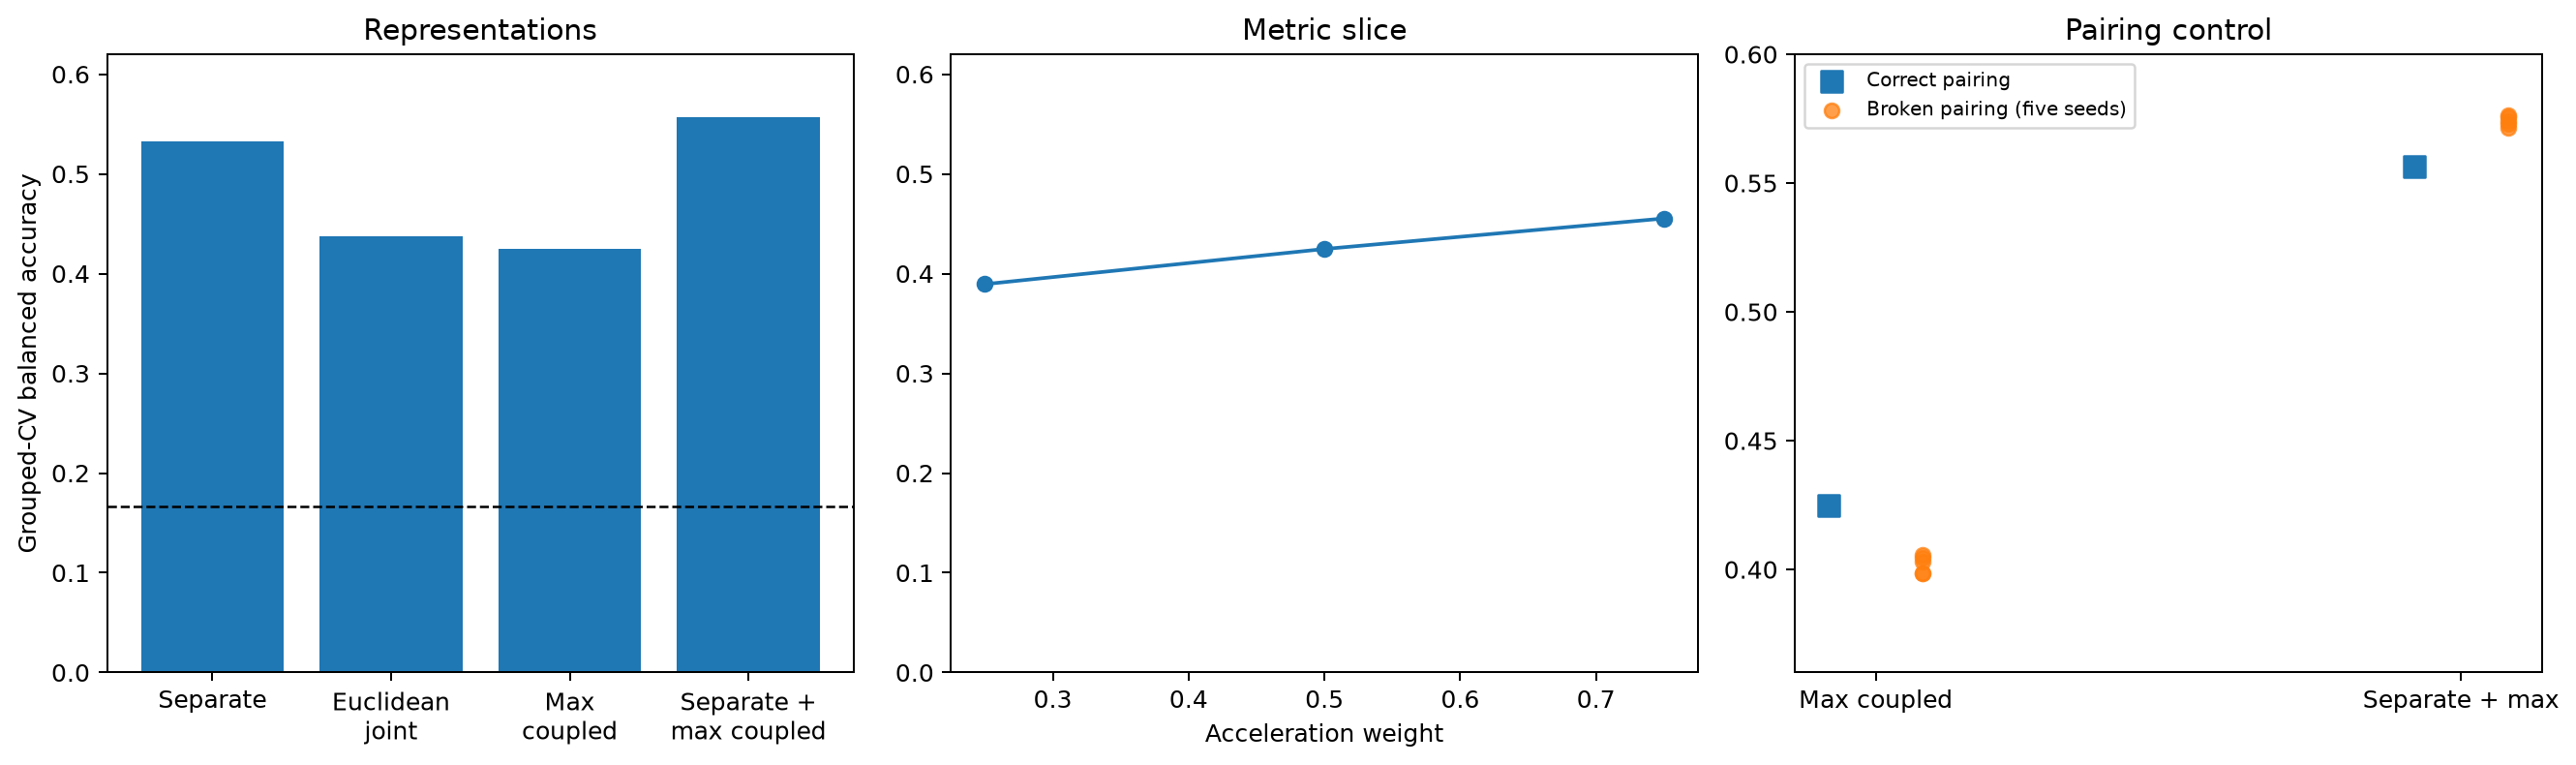
\includegraphics[width=\textwidth]{coupled_max_filtration.png}
\caption{Development-only max-coupled analysis. Left: comparison with the separate and Euclidean-joint representations. Middle: one-parameter slices of the acceleration--gyroscope bifiltration. Right: correct pairing and five marginal-preserving derangements.}
\label{fig:max-coupled}
\end{figure}

Correct pairing scores 0.425 when the max-coupled vector is used alone, whereas five broken-pairing realizations score 0.398--0.406. For the declared seed, the subject-level correct-minus-broken mean is 0.027 with interval $[-0.006,0.058]$. After appending separate topology, correct pairing scores 0.557 and the broken realizations score 0.571--0.576; the corresponding mean difference is $-0.014$ with interval $[-0.029,0.001]$. Requiring closeness in both sensors does not change the conclusion: the classification gain is not evidence of correct sensor synchronization.

\section{Discussion}

Delay-cloud stable ranks contain activity information that transfers across subjects. Between-activity prototypes are farther apart than same-activity prototypes across people, the dendrogram separates static from dynamic activities, and the observed prototype score exceeds all 2,000 permutation scores.

Time shuffling preserves every sensor value but changes which delayed measurements occupy the same point. Its 0.503 test score, compared with 0.580 in the correct order, shows that temporal adjacency contributes to the result. This is not recovery of directed dynamics: complete reversal leaves delay persistence unchanged. The smaller delay-minus-instantaneous difference is inconclusive.

The circular-coordinate branch turns one persistent $H_1$ class into an ordered phase variable. Its rate and linearity separate the three repeated motions from the static postures, while loop lifetimes also distinguish walking, upstairs, and downstairs. This provides an interpretable topological result for all six activities rather than relying on selected example trajectories. The association with Fourier frequency is positive but moderate, as expected because the methods measure different objects.

The 16 topological-dynamics features outperform the 256 stable-rank samples, but their concatenation is worse than the concise vector alone. Stable rank discards birth scales and which bar generated which lifetime; it also contains no ordering of a cocycle coordinate. Conversely, the new vector explicitly keeps the longest-loop birth and lifetime and relates its circular coordinate back to time. The two representations are therefore partly redundant, while the larger concatenation is harder to estimate from 21 development subjects.

Both topological representations remain far behind the conventional baselines, and concatenation of stable ranks with compact summaries hurts performance. Restoring two RMS radii raises stable-rank balanced accuracy to 0.640, so both normalized shape and movement magnitude carry activity information.

\pagebreak
The Euclidean and max-product coupled clouds are less predictive than the two separate clouds, but appending either vector improves mean subject-level performance. Breaking the pairing leaves this improvement intact and often increases it slightly. Since both marginal clouds remain unchanged, the gain cannot be assigned to synchronization. Both coupled constructions are post-hoc and use development subjects only.

A 2.56-second window contains only a few gait cycles, which limits both loop persistence and frequency resolution. Sitting, standing, and laying also depend strongly on gravity and device orientation in the supplied UCI features, while our topology uses body acceleration and removes global scale.

The scope is limited to one phone placement, 30 adults, scripted activities, and presegmented windows without transition classes. Windows overlap, although subject-level splitting and bootstrapping prevent this dependence from crossing evaluation units. The delay choice uses mean linear autocorrelation; mutual information or false-nearest-neighbor criteria could provide alternatives. Only $H_0$ and $H_1$ are used. The cityblock thresholds are discretized on a separate fixed range, so metric performance is a robustness check rather than a perfectly matched filtration-scale comparison.

Future work should test richer but still stable summaries, especially persistence images or kernels that retain the whole birth--death distribution. Circular coordinates could also be aligned across overlapping windows to study phase continuity beyond the present window-level regression. The max-coupled analysis uses only three one-parameter slices; a full two-parameter rank invariant could study the acceleration--gyroscope bifiltration without selecting one sensor balance in advance. Any extension should keep the same subject-disjoint protocol and compare against the strong 561-feature reference.

\section{Reproducibility}

All computations use Python 3.13, NumPy 2.5.3, Ripser.py 0.6.15, StableBear 0.4.3, Matplotlib 3.11.2, and scikit-learn 1.9.1. Random operations use seed 2956. The complete workflow is:

\begin{verbatim}
python -m unittest -v test_analysis.py
jupyter nbconvert --to notebook --execute --inplace analysis.ipynb \
  --ExecutePreprocessor.timeout=-1
python make_figures.py
\end{verbatim}

The notebook is the single analysis entry point. In the order presented, it calls four named functions from \texttt{experiments.py}: the primary comparison, robustness checks, coupling and ablation extensions, and circular-coordinate dynamics. Those functions contain reusable caching and repeated computation, while the notebook exposes every experiment call and interprets its output. Setting \texttt{RECOMPUTE=True} refits every model and refreshes the saved JSON results; the default reuses verified results and expensive feature caches. \texttt{make\_figures.py} only exports the already analysed results as report images.

\clearpage
\section{Conclusion}

Delay embedding and persistent homology recover activity structure that transfers to unseen subjects. Time shuffling lowers stable-rank performance, showing that temporal adjacency matters. More importantly, the longest persistent $H_1$ class yields a circular coordinate whose rate, linearity, birth, and lifetime form an interpretable 16-feature description of all six activities. It reaches 0.611 test balanced accuracy, compared with 0.580 for sampled stable ranks, while combining the two does not improve it. Euclidean and max-product couplings add coordinates but do not establish sensor synchronization because broken pairings perform as well. Ordinary features remain much stronger. The TDA is therefore useful here as a compact description of motion geometry and periodic phase, not as the best activity classifier.

\begingroup
\small
\setlength{\itemsep}{0.35em}
\begin{thebibliography}{9}

\bibitem{course-notes}
W. Chacholski.
\newblock \emph{Analysis pipeline: SF2956 Topological Data Analysis course notes}.
\newblock KTH Royal Institute of Technology.

\bibitem{uci-paper}
D. Anguita, A. Ghio, L. Oneto, X. Parra, and J. L. Reyes-Ortiz.
\newblock A public domain dataset for human activity recognition using smartphones.
\newblock In \emph{ESANN}, 2013.

\bibitem{uci-repository}
UCI Machine Learning Repository.
\newblock Human Activity Recognition Using Smartphones, dataset 240.
\newblock \url{https://archive.ics.uci.edu/dataset/240/human+activity+recognition+using+smartphones}.

\bibitem{takens}
F. Takens.
\newblock Detecting strange attractors in turbulence.
\newblock In \emph{Dynamical Systems and Turbulence, Warwick 1980}, Lecture Notes in Mathematics 898, pp. 366--381, 1981.

\bibitem{ripser}
U. Bauer.
\newblock Ripser: efficient computation of Vietoris--Rips persistence barcodes.
\newblock \emph{Journal of Applied and Computational Topology}, 5:391--423, 2021.

\bibitem{ripserpy}
C. Tralie, N. Saul, and R. Bar-On.
\newblock Ripser.py: a lean persistent homology library for Python.
\newblock \emph{Journal of Open Source Software}, 3(29):925, 2018.

\bibitem{stablebear}
B. Wehlin.
\newblock StableBear 0.4.3 documentation.
\newblock \url{https://docs.stablebear.org/en/v0.4.3/}.

\bibitem{stable-rank}
W. Chach\'olski and H. Riihim\"aki.
\newblock Metrics and stabilization in one parameter persistence.
\newblock \emph{SIAM Journal on Applied Algebra and Geometry}, 4(1):69--98, 2020.

\bibitem{circular-coordinates}
V. de Silva, D. Morozov, and M. Vejdemo-Johansson.
\newblock Persistent cohomology and circular coordinates.
\newblock \emph{Discrete \& Computational Geometry}, 45:737--759, 2011.

\bibitem{scikit-learn}
F. Pedregosa et al.
\newblock Scikit-learn: machine learning in Python.
\newblock \emph{Journal of Machine Learning Research}, 12:2825--2830, 2011.

\end{thebibliography}
\endgroup

\end{document}
